% Supplementary material to "Global minimality of controlled-rail brachistochrones in conformal
% Kerr and Vaidya spacetimes". Build: see README.md in this folder.
\documentclass[aip,jmp,amsmath,amssymb,reprint]{revtex4-2}
\usepackage{amsmath}
\usepackage{amsthm}
\usepackage{xcolor}
\usepackage{graphicx}
\usepackage{xr-hyper}
\usepackage{hyperref}
\setlength{\emergencystretch}{2em}

\newcommand{\Ehat}{\hat E}
\newcommand{\dd}{\mathrm{d}}
\newcommand{\gopt}{g_{\rm opt}}
\renewcommand{\theenumi}{\arabic{enumi}}
\renewcommand{\labelenumi}{(\theenumi)}
\newcommand{\todo}[1]{\textcolor{red}{[TODO: #1]}}

\theoremstyle{plain}
\newtheorem{theorem}{Theorem}
\newtheorem{proposition}{Proposition}[section]
\newtheorem{lemma}[proposition]{Lemma}
\newtheorem{corollary}[proposition]{Corollary}
\newtheorem{fact}[proposition]{Fact}
\theoremstyle{definition}
\newtheorem{definition}[proposition]{Definition}
\newtheorem{remark}[proposition]{Remark}

\externaldocument[M-]{paper3}
\renewcommand{\thesection}{S\arabic{section}}

\begin{document}

\title{Supplementary material to ``Global minimality of
controlled-rail brachistochrones in conformal Kerr and Vaidya spacetimes'': alternative proofs and
computer-assisted steps}
\author{Iman Rosignoli}
\affiliation{Department of Physics, University of Pavia, Via A.\ Bassi 6, 27100 Pavia, Italy}
\maketitle

\section{Scope}
\label{sec:supp-scope}
This supplement contains material that the main text uses or announces but does not print in full. References
of the form ``main text'' are to the numbering of the paper; the sections follow its order.

Sections~\ref{sec:frames}--\ref{sec:family} give an alternative proof of the cut-point rule for conformal
Schwarzschild (Theorem~\ref{M-thm:angle} of the main text) on narrower ranges of $q$, by convex wavefronts on
Hadamard slices in static conformal frames. The convex-front argument is not needed for the main-text
cut-point results, whose proofs use the comparison of Lemma~\ref{M-lem:tk-sturm} and the count of
Proposition~\ref{M-prop:count}. Where it applies, this proof also excludes meetings of distinct null rays in
the universal cover of the plane at every swept angle. It works directly on a time interval that need not
contain the whole future; finite-window minimality is also established in the main text by
Corollary~\ref{M-cor:finite-window}.

The remaining sections contain the computer-assisted steps and the constants of the examples:
section~\ref{sec:supp-sharp32} the constants of the sharpness example below $q=3/2$;
section~\ref{sec:supp-kerr-cert} the curvature certificates on the equator of Kerr;
section~\ref{sec:supp-tau-cert} the certified critical separations and the Maxwell example of the proper-time
branch; section~\ref{sec:supp-ts-examples} the examples with a time-dependent factor;
section~\ref{sec:supp-tk-example} the proofs with constants in the example on the equator with spin; and
section~\ref{sec:supp-vaidya} the constants of the Vaidya example. In each case the main text states the
result and the structure of its proof. Scripts, logs and certificate files are in the accompanying repository.

\section{Static conformal frames}
\label{sec:frames}
In the plane the auxiliary spacetime is three-dimensional. Its Weyl tensor vanishes and
the screen of a null geodesic is one-dimensional, so the in-plane Jacobi equation is
\begin{equation}
  y''+\mathrm{Ric}(k,k)\,y=0
  \label{eq:jacobi-3d}
\end{equation}
in an affine parameter. Null conjugate points are conformally invariant, and we use
conformal frames in which the slices carry a \emph{static} metric. For a constant
$b\in[3/2,\infty]$ let
\begin{equation}
  N_b=\Big(1-\frac fb\Big)^{-1}\ (N_\infty=1),\qquad
  \bar g_b=\frac{N_b}{N}\,\gopt=-N_bV^2\,\dd\eta^2+N_b\,h_0 .
  \label{eq:gb}
\end{equation}
The frame $\bar g_b$ does not freeze $A$: it is another conformal representative of the
same null cone, with slice metric $h_b=N_bh_0$ independent of $\eta$.

\begin{lemma}[no time derivatives]\label{lem:static-frame}
For a metric $-\tilde V(\eta,x)^2\dd\eta^2+\tilde h(x)$ with $\tilde h$ independent of
$\eta$, and $k=(1,\tilde V e)$ with $|e|_{\tilde h}=1$,
\begin{equation}
  \mathrm{Ric}(k,k)=\tilde V^2K_{\tilde h}+\tilde V\,\mathrm{Hess}_{\tilde h}\tilde V(e_\perp,e_\perp),
  \label{eq:ric-static}
\end{equation}
with $e_\perp$ the $\tilde h$-unit vector orthogonal to $e$. In particular
$\mathrm{Ric}_{\bar g_b}(k,k)$ depends on $\eta$ only through the value $q(\eta)$, not
through $A'$ or $A''$.
\end{lemma}

\begin{proof}
For such a metric $R_{00}=\tilde V\Delta_{\tilde h}\tilde V$, $R_{0i}=0$ and
$R_{ij}=R_{\tilde h,ij}-\tilde V^{-1}\mathrm{Hess}_{\tilde h}\tilde V_{ij}$: the time
derivatives of $\tilde V$ cancel. In two spatial dimensions
$R_{\tilde h}=K_{\tilde h}\tilde h$, and contracting with $k$ gives~\eqref{eq:ric-static}.
For $\bar g_b$, $\tilde V^2=N_b(1-f/q)$ and $\tilde h=N_bh_0$.
\end{proof}

The normalization $k^\eta=1$ is not affine; for an affine tangent the contraction is
multiplied by $(\dd\eta/\dd\lambda)^2>0$, which does not change its sign. Writing
$e=\cos\alpha\,e_r+\sin\alpha\,e_\varphi$ in an $h_0$-orthonormal frame,
$\mathrm{Ric}_{\bar g_b}(k,k)=C_r\cos^2\alpha+C_\varphi\sin^2\alpha$.

\begin{proposition}[sign certificates]\label{prop:certificates}
Write $R=r/M=2+x$, $x>0$. Then $\mathrm{Ric}_{\bar g_b}(k,k)<0$ for every null direction
and every $r>2M$ in each of the following cases.
\begin{enumerate}
\item $b=\infty$ and $q\ge2$. Here
  $C_r=-M\{Mq+(2q-1)(r-2M)\}/(qr^4)$ and $C_\varphi=-MP/\{qr^5[2M+(q-1)r]\}$, where, with
  $q=2+d$, $d\ge0$,
  \[
    M^{-3}P=(2d^2+2d)x^3+(9d^2+24d+12)x^2+(12d^2+48d+48)x+4d^2+16d+16 .
  \]
\item $b=2$ and $q\ge5/3$. Here $C_r=-P_r/[M^2qR^5(R+2)^2]$,
  $C_\varphi=-P_\varphi/[M^2qR^5(R+2)((q-1)R+2)]$ with
  \begin{align*}
    P_r&=x^4+(12q-4)x^3+(72q-36)x^2+(112q-32)x+32q,\\
    P_\varphi&=(3q-5)(q-1)x^4+(20q^2-37q+14)x^3\\
    &\quad+(48q^2-42q)x^2+48q^2x+16q^2 .
  \end{align*}
\item $b=5/3$ and $11/7\le q\le2$. Here $C_r=-Q_r/[4M^2qR^5(R+3)^2]$,
  $C_\varphi=-Q_\varphi/[2M^2qR^5(R+3)((q-1)R+2)]$ with
  \begin{align*}
    Q_r&=4(2-q)x^4+(37q-3)x^3+(390q-210)x^2+(700q-200)x+200q,\\
    Q_\varphi&=(7q-11)(q-1)x^4+(47q^2-87q+34)x^3\\
    &\quad+(114q^2-102q)x^2+116q^2x+40q^2 .
  \end{align*}
\item $q$ constant, $b=q\ge3/2$ (ultrastatic frame). Here $\mathrm{Ric}(k,k)=K_t$, the
  optical Gauss curvature of Paper~II, and with $q=3/2+d$ the numerator of $-K_t$ is
  \[
    2d^2x^3+9d^2x^2+12d^2x+4d^2+dx^3+16dx^2+34dx+12d+\tfrac{23}{4}x^2+24x+9 .
  \]
\end{enumerate}
In each case all coefficients are non-negative and the constant term is positive on the
stated range of $q$ (for $20q^2-37q+14$ and $47q^2-87q+34$, check the lower end of the
range and monotonicity).
\end{proposition}

\begin{proof}
Direct computation from~\eqref{eq:ric-static}, verified symbolically by the scripts
\texttt{supplement\_*.wls} of the accompanying repository (the four cases and the frames; the file
\texttt{RESULTS\_MAP.md} there gives the script of each step).
\end{proof}

\begin{remark}[sharpness of the frames]\label{rmk:frames-sharp}
The certificates are frame-dependent sufficient conditions, not thresholds for
minimality. In the frame $b=\infty$, $\lim_{r\to\infty}r^3C_\varphi=-2M(q-2)/q$, so the sign
fails far out for $q<2$; in the frame $b=2$ it fails far out for $q$ just below $5/3$, and
in the frame $b=5/3$ for $q$ just below $11/7$. For constant $q$ the threshold $3/2$ of
item~4 is exactly that of Paper~II. The frame must be fixed along the whole extremal:
switching $b$ in time would destroy the static slice metric that the next two lemmas use.
\end{remark}

\begin{lemma}[Hadamard slices]\label{lem:hadamard}
For $b\in[3/2,\infty]$ the universal cover of $(\{r>2M\}\times S^1,h_b)$, with the angle
unwrapped, is a Hadamard surface: complete, simply connected, with $K_{h_b}<0$.
\end{lemma}

\begin{proof}
$K_{h_b}$ is the optical curvature $K_t$ at constant $q=b$, negative by
Proposition~\ref{prop:certificates}(4); for $b=\infty$,
$K_{h_0}=M(3M-2r)/r^4<0$. The radial integrand $\sqrt{N_b}/f$ behaves as $2M/(r-2M)$ at the
inner end and tends to a positive constant at infinity, so radial distances diverge at
both ends; and $N_b\ge1$ with $r^2/f-27M^2=(r-3M)^2(r+6M)/(r-2M)\ge0$ bounds the angular
radius below by $3\sqrt3M$. A curve of finite length therefore escapes neither radially
nor in the unwrapped angle.
\end{proof}

\section{Positive expansion, convex fronts, no crossing}
\label{sec:fronts}
Fix a frame $\bar g_b$ in which Proposition~\ref{prop:certificates} applies along the
time interval considered. Let $F_t:S^1\to\tilde S_t$ be the \emph{front}: $\alpha\mapsto$
the position at $\eta=t$ of the null geodesic from the (lifted) launch event $\tilde o$
with initial direction $\alpha$, in the universal cover $\tilde S$ of the slice.

\begin{lemma}[expansion]\label{lem:expansion}
Along every null geodesic of the cone of $\tilde o$, the in-plane Jacobi field $y$ with
$y(0)=0$, $y'(0)>0$ satisfies $y\ge y'(0)\lambda$ and $\theta=y'/y\ge1/\lambda>0$.
\end{lemma}

\begin{proof}
While $y>0$, $y''=-\mathrm{Ric}(k,k)y\ge0$, so $y'\ge y'(0)$ and $y\ge y'(0)\lambda$: there
is no first zero. Moreover $(\lambda y'-y)'=\lambda y''\ge0$, so $\lambda y'\ge y$.
\end{proof}

\begin{lemma}[convex fronts]\label{lem:fronts}
Each $F_t$ is an immersion, it moves along its $h_b$-normal with speed $\tilde V>0$, and
its geodesic curvature with respect to the direction of motion is positive.
\end{lemma}

\begin{proof}
The variation at fixed $\eta$ is $Y+c_1k$, with $Y$ the Jacobi field of the cone; since
$\bar g_b(Y,k)=0$, $|\partial_\alpha F_t|^2_{h_b}=\bar g_b(Y,Y)=y^2>0$. The spatial velocity
$v$ of a ray satisfies $h_b(v,\partial_\alpha F_t)=\bar g_b((0,\partial_\alpha F_t),k)=0$ and
$|v|_{h_b}=\tilde V$. For a normal flow in a static metric,
$\partial_t\log|\partial_\alpha F_t|_{h_b}=\tilde V\kappa$, and the left side is
$\theta/(\dd\eta/\dd\lambda)>0$ by Lemma~\ref{lem:expansion}.
\end{proof}

\begin{lemma}[no crossing in the universal cover]\label{lem:nocross}
Two distinct null geodesics from $\tilde o$ do not meet.
\end{lemma}

\begin{proof}
On the cover every slice is a Cauchy surface: causal curves have
$|\dd x/\dd\eta|_{h_b}\le\tilde V$, bounded on compact time intervals, and $h_b$ is complete
(Lemma~\ref{lem:hadamard}). Let $R_t=J^+(\tilde o)\cap\tilde S_t$: compact, with interior
containing the launch point, non-decreasing in $t$ (the lines $L_x$ are timelike), and
$\partial R_t\subset F_t(S^1)$ because $\partial J^+(\tilde o)$ is generated by null
geodesics from $\tilde o$.

Suppose a crossing exists and let $t_*$ be the first time at which $F_t$ fails to be
injective; it is attained with two distinct directions, because the immersion is
uniform on compact sets. For $t<t_*$, $F_t$ is a Jordan curve and $R_t$ is the closed disk
it bounds, with outward direction of motion. By Lemma~\ref{lem:fronts} its boundary has
positive curvature, so $R_t$ is locally geodesically convex, hence convex on the Hadamard
surface: a shortest curve inside the disk between two of its points is an ambient
geodesic, hence the unique segment.

The limit body $R_{t_*}=\overline{\bigcup_{t<t_*}R_t}$ is compact and convex with
non-empty interior, and $F_{t_*}(S^1)=\partial R_{t_*}$: a limit of earlier boundary
points that were interior to the limit body would lie inside a small geodesic triangle
with vertices in the union, hence inside some $R_s$, $s<t_*$, by convexity. The boundary
of a compact convex body with interior in a Hadamard surface is a topological circle;
$F_{t_*}$ is an immersion onto it, hence a covering, and its degree about the launch
point is one, as for the earlier simple fronts. A covering of degree one is injective,
contradicting the choice of $t_*$.
\end{proof}

\section{The theorem in static frames}
\begin{proposition}[convex fronts]\label{prop:angle-frames}
Assume (H1) and one of the following on the whole of $I$:
\begin{equation}
  \mathrm{(a)}\ q(\eta)\ge2;\qquad \mathrm{(b)}\ q(\eta)\ge\tfrac53;\qquad
  \mathrm{(c)}\ \tfrac{11}{7}\le q(\eta)\le2;\qquad
  \mathrm{(d)}\ A\ \text{constant and}\ q\ge\tfrac32 .
  \label{eq:bands}
\end{equation}
Then the fronts of section~\ref{sec:fronts} are convex in a static frame, two distinct null
geodesics from $\tilde o$ never meet in the universal cover (Lemma~\ref{lem:nocross}), and
the same minimality and cut-point conclusions as in Theorem~\ref{M-thm:angle} hold throughout $I$,
by the argument below; here $I$ need not contain the whole future.
\end{proposition}

\begin{proof}
Choose the frame $b=\infty,2,5/3$ or $q$ in cases (a)--(d). By
Proposition~\ref{prop:certificates} and Lemma~\ref{lem:expansion} there is no in-plane
conjugate point, and by Lemma~\ref{M-lem:outofplane} the first out-of-plane one is at
$\Delta\varphi=\pi$. Suppose $\gamma$ had a cut point before $\pi$. It is not conjugate, so
by Fact~\ref{M-fact:cut}(4) a second maximal null geodesic $\sigma$ from $o$ reaches the same
event. Being maximal, $\sigma$ has swept angle at most $\pi$. For $0<\Delta\varphi<\pi$ the
center, the launch point and the end point fix a unique plane; the opposite sense would
need $2\pi-\Delta\varphi>\pi$, and further windings more. So $\sigma$ lies in the plane of
$\gamma$, with the same sense and the same unwrapped angle, and $\gamma$, $\sigma$ lift to
null geodesics from $\tilde o$ meeting at the same point of the cover, which
Lemma~\ref{lem:nocross} excludes. Hence every event before $\pi$ is on
$\partial J^+(o)$, reached by a unique null segment, and Theorem~\ref{M-thm:schw} gives
items~1--2. At $\Delta\varphi=\pi$ the event stays on the causal boundary by continuity
($I^+(o)$ is open), and the rotations of Lemma~\ref{M-lem:outofplane} give a family of
distinct minimizers: it is the first cut point. Beyond it the conjugate point is
interior, the segment is no longer achronal, and an earlier arrival exists.

For a radial extremal the rotations fix it and the argument above does not apply. Every
causal competitor obeys $|\dd r/\dd\eta|\le fV$, while the radial extremals solve
$r'=\pm fV$. For the outgoing branch $w=R-r$ satisfies $w'=a(\eta)w+d(\eta)$ with $a$
bounded on the compact set traversed and $d=fV-r'\ge0$; an integrating factor gives
$w\ge0$, with $w>0$ at arrival unless $d=0$ almost everywhere, which forces saturation of
the radial speed and zero angular velocity. The ingoing branch is analogous, and radial
completeness prevents reaching $r=2M$ or infinity in finite time.
\end{proof}

Lemma~\ref{lem:nocross} excludes meetings of distinct rays in the cover at every swept
angle, not only below $\pi$; the uniqueness proved in section~\ref{M-sec:angle-proof} is the
weaker statement needed for Theorem~\ref{M-thm:angle}.

\section{The whole family of static frames}
\label{sec:family}
Cases (a)--(c) of Proposition~\ref{prop:angle-frames} are three frames of a one-parameter family. For a
constant $b>3/2$, write the negatives of the numerators of $C_r$ and $C_\varphi$ in the frame
$\bar g_b$ (with $M=1$, $r=2+x$; the denominators $qr^5(2+(b-1)r)^2$ and
$qr^5(2+(b-1)r)(2+(q-1)r)$ are positive):
\begin{align*}
P_r={}&(b-1)(2bq-b-4q+3)x^4+(13b^2q-6b^2-24bq+11b+8q-2)x^3\\
&+6b(5bq-2b-4q+1)x^2+4b^2(7q-2)x+8b^2q,\\
P_\varphi={}&(q-1)(2bq-4b-q+3)x^4+(13bq^2-24bq+8b-6q^2+11q-2)x^3\\
&+6q(5bq-4b-2q+1)x^2+4q^2(7b-2)x+8bq^2 .
\end{align*}

\begin{proposition}[the band of a frame]\label{prop:family}
For $b,q\ge3/2$ the coefficients of $x^0,\dots,x^3$ in $P_r$ and $P_\varphi$ are positive.
The coefficients of $x^4$ are non-negative exactly when
\begin{equation}
  q_-(b):=\frac{4b-3}{2b-1}\ \le\ q\ \le\ q_+(b):=
  \begin{cases}\dfrac{3-b}{4-2b},& b<2,\\[1ex] +\infty,& b\ge2.\end{cases}
  \label{eq:band}
\end{equation}
Hence $\mathrm{Ric}_{\bar g_b}(k,k)<0$ for every $r>2M$ and every null direction if and only
if $q$ lies in~\eqref{eq:band}; outside it the sign fails at large $r$.
\end{proposition}

\begin{proof}
With $b=3/2+u$, $q=3/2+v$ each coefficient of degree $0$--$3$ is a polynomial in $u,v$ with
positive coefficients; for instance the radial $x^3$ coefficient is
$13u^2v+\tfrac{27}{2}u^2+15uv+\tfrac{31}{2}u+\tfrac54v+\tfrac{23}{8}$, and the tangential one
follows by exchanging $u$ and $v$. The $x^4$ coefficients are non-negative iff
$(2b-4)q+3-b\ge0$ and $(2b-1)q+3-4b\ge0$; for $b\ge2$ the first is automatic, since at
$q=q_-(b)$ it equals $3(b-1)(2b-3)/(2b-1)>0$. When an $x^4$ coefficient vanishes the
constant term is still positive. The asymptotics
$\lim_{r\to\infty}r^3C_r=-(3-b-4q+2bq)/((b-1)q)$ and
$\lim_{r\to\infty}r^3C_\varphi=-(3-4b-q+2bq)/((b-1)q)$ give the converse.
\end{proof}

The bands are exact for this criterion and this family of frames, not thresholds for
minimality. Since $q_\pm'(b)=2/(2b-1)^2,\ 2/(4-2b)^2>0$, the best frame for a range
$[q_{\min},q_{\max}]$ is the largest $b$ with $q_-(b)\le q_{\min}$, namely
$b_*=(3-q_{\min})/(4-2q_{\min})$ for $q_{\min}<5/3$, and $q_+(b_*)=(9-5q_{\min})/(10-6q_{\min})$.

\begin{proposition}[continuous family of frames]\label{thm:C}
Assume (H1), and let $q_{\min}=\inf_Iq$, $q_{\max}=\sup_Iq$. If
\[
  q_{\min}\ge\tfrac53,\qquad\text{or}\qquad
  \tfrac32<q_{\min}<\tfrac53\ \ \text{and}\ \ q_{\max}\le\frac{9-5q_{\min}}{10-6q_{\min}},
\]
then $\mathrm{Ric}(k,k)<0$ in a static frame, the fronts are convex, and two distinct null
geodesics from $\tilde o$ never meet in the universal cover, for an arbitrary $C^2$ factor.
\end{proposition}

\begin{proof}
Use the frame $\bar g_{b_*}$ ($b=2$ if $q_{\min}\ge5/3$): Proposition~\ref{prop:family} gives
$\mathrm{Ric}(k,k)<0$, Lemma~\ref{lem:hadamard} gives Hadamard slices, and
Lemmas~\ref{lem:expansion}--\ref{lem:nocross} apply verbatim.
\end{proof}

Proposition~\ref{thm:C} contains cases (a)--(c), and every $q_0>3/2$ has a non-constant band
around it: $q_{\min}=1.55$ allows $q_{\max}\le1.786$, $q_{\min}=1.6$ allows $q_{\max}\le2.5$,
$q_{\min}=1.65$ allows $q_{\max}\le7.5$. A single frame must work on the whole time interval.


\begin{figure}[t]
\centering
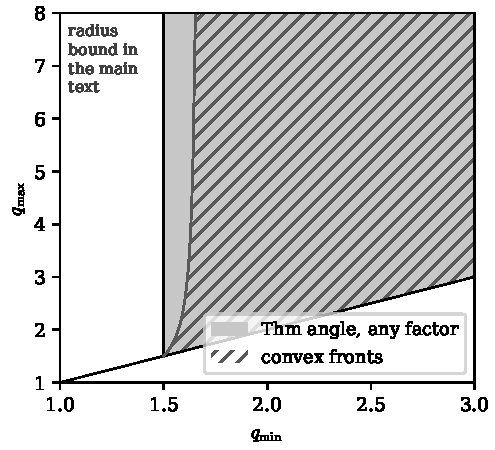
\includegraphics[width=0.6\textwidth]{../figures/fig2_bands_supplement.pdf}
\caption{Arrival branch, $a=0$, in the $(q_{\min},q_{\max})$ plane: Theorem~\ref{M-thm:angle} of the
main text covers $q_{\min}\ge3/2$ for an arbitrary smooth factor (grey); hatched, the narrower ranges
where the convex-front argument of Propositions~\ref{prop:angle-frames} and~\ref{thm:C} also
applies.}
\label{fig:bands-frames}
\end{figure}

\section{Constants in the sharpness example}
\label{sec:supp-sharp32}
This section verifies the constants stated for $q=6/5$ in Proposition~\ref{M-prop:sharp32}. Here
$A_1=-3\sqrt6$ and, with $x=M/r$, $F=\sqrt{1-2x}\,(1+10x)/(1+12x-40x^2)$ in \eqref{M-eq:fermat-plane}. The
substitution $\sqrt{1-2x}=(p^2-12p+30)/(p^2-10p+30)$, $\sqrt{1+10x}=(30-p^2)/(p^2-10p+30)$, $0\le p\le11/10$, covers
$r\ge10M$ monotonically and makes $\rho^2G/M^2$ and $-\rho^3G'/M^2$ rational in $p$. The non-negativity of
$\rho^2G$, $465M^2-\rho^2G$, $-\rho^3G'$ and $930M^2+\rho^3G'$ on that interval follows from the signs of the
Bernstein coefficients of their numerators and denominators, computed in exact rational arithmetic. So
\eqref{M-eq:G-bounds} holds with $K=465$ and $\rho_*=\rho(10M)$. With $D\ge D_0=2\times10^4M$ and
$b_\pm=\beta_\pm\sqrt{D/D_0}$, $\beta_-=300M$, $\beta_+=2000M$, put $t=D/D_0\ge1$, so that
$b_\pm^2/D^2=\beta_\pm^2/(D_0^2t)\le\epsilon_\pm$ with $\epsilon_-=9/40000$ and $\epsilon_+=1/100$. Since $D_0>KM/c$,
$0<F_{\min}:=1-cM/D_0-KM^2/D_0^2\le F(D)\le1$. Moreover $\rho_*=5\sqrt{15}\,M<20M$ and
$b_c\le\rho(3M)=\sqrt{486/13}\,M<7M$, so $b_\pm\ge300M>\max(\rho_*,b_c)$ and the bounds of the proof of
Proposition~\ref{M-prop:sharp32} apply. Write $s_\pm(t)=\sqrt{1-\epsilon_\pm/t}$. For the lower bound,
$F(D)\le1$, $\sqrt{1-\epsilon_-}\le s_-(t)\le1$ and $D|R_1|\le\pi KM^2D_0/(\beta_-^3\sqrt t)$ are used; for the upper
bound, $F(D)/s_+(t)\ge F_{\min}$, $s_+(t)\le1$ and $t^{-1/2}\le1$. With $c=3\sqrt6$ this gives
\[
  D\Phi_b(b_-)\ge-\frac2{\sqrt{1-\epsilon_-}}+\frac{2cMD_0\sqrt{1-\epsilon_-}}{\beta_-^2}-\frac{\pi KM^2D_0}{\beta_-^3}>0.1832,
\]
\[
  D\Phi_b(b_+)\le-2\Big(1-\frac{cM}{D_0}-\frac{KM^2}{D_0^2}\Big)+\frac{2cMD_0}{\beta_+^2}+\frac{\pi KM^2D_0}{\beta_+^3}<-1.922 .
\]
Moreover $b_+\le D/2$ for $t\ge1$ and $b_-\ge300M>\pi KM/(2\sqrt3\,c)$, so $\Phi<\pi$ on $[b_-,b_+]$; and
$\rho(8200M)^2=6\cdot8200^4M^2/(8198\cdot8210)>D_0^2$.

\section{Curvature certificates on the equator}
\label{sec:supp-kerr-cert}
This section describes the certificates behind Propositions~\ref{M-prop:kerr-Kinf} and~\ref{M-prop:kerr-Kvar}
and the radial confinement of the rays in case~(2) of the latter. Each certificate is a closed algebraic
lemma: a sign condition for a polynomial with rational coefficients on a box $[0,1]^d$, together with its
proof. The polynomials are, up to an explicit positive factor, the geometric inequalities of the main text
written in the box variables; this identification is a separate symbolic computation (see the last
paragraph).

\paragraph{Positivity on a cell.} On a cell of a binary subdivision of $[0,1]^d$, rescaled to the unit box,
a polynomial is written in the tensor Bernstein basis of its multidegree. If all Bernstein coefficients are
positive (non-negative), the polynomial is positive (non-negative) on the cell. A certificate of this kind
is a subdivision tree, read in preorder, whose nodes are bisections along a named axis and whose leaves
are cells where the criterion holds. The leaves cover the box by construction.

\paragraph{Inequalities with one square root.} Several inequalities have the form $P_0+P_1\sqrt g\ge0$ with $g\ge0$.
On a leaf, let $g_0$ and $g_1$ be the smallest and the largest Bernstein coefficient of $g$ (with $g_0$
replaced by $0$ if negative), so that $g_0\le g\le g_1$ there. Two affine bounds for $v=\sqrt g$ are used:
the chord through $(g_0,s_0)$ and $(g_1,s_1)$, with rationals $s_0^2\le g_0$, $s_1^2\le g_1$, which lies below
$\sqrt g$ by concavity, and the tangent bound $\sqrt g\le\sigma/2+g/(2\sigma)$ for a rational $\sigma>0$. Since
$P_0+P_1v$ is affine in $v$, it suffices that $P_0+AP_1+BP_1g$ has non-negative Bernstein coefficients for
the two pairs $(A,B)$ given by these lines. A second form avoids the envelopes: with
$Q=P_1^2g-P_0^2$, on each leaf one of the sets $\{P_0\ge0,P_1\ge0\}$, $\{P_1\ge0,Q\ge0\}$, $\{P_0\ge0,-Q\ge0\}$ is
certified, and each implies the inequality.

\paragraph{The certificates.} Table~\ref{tab:kerr-cert} lists them, $33$ in all. The box variables are
affine images of the physical ones, except where stated: $u=1/q$, $t=\tan(\alpha/2)$ for the direction of the
null vector, and $R=r_+/M$ with $a^2=R(2-R)$.
\begin{enumerate}
\item \emph{Static part, constant factor} (used in Proposition~\ref{M-prop:kerr-Kvar}(1) for $R_{\rm stat}<0$):
  box $(X,U,Z)$ with $x=2M/r=X$, $u=U/2$, $a^2/M^2=\frac{1089}{2500}Z$, that is $q\ge2$ and $|a|\le33M/50$. Four
  non-negativity lemmas, one cell each; together they give $U\le0$, $V\le0$, $V^2\ge J^2$ and $J^2\le4U^2$ for
  $\mathrm{Ric}=U(1-s^2)+Vs^2+Js$, hence $\max_{s\in[-1,1]}\mathrm{Ric}\le0$.
\item \emph{Proposition~\ref{M-prop:kerr-Kinf}}: box $(X,R_v,U)$ with $x=r_+/r=X$, $R=1+R_v$, $u=\frac35U$. One
  certificate with three sufficient sets on its $19$ leaves: $\{V\le0,\ V^2\ge J^2\}$ together with one of
  $J^2\le-4U(U-V)$ (the value at the vertex is non-positive), $V\ge U$ (the quadratic in $s$ is convex), or
  $\{U\le0,\ J^2\le U^2\}$. Each set implies $\max_s\mathrm{Ric}\le0$; this implication is part of the proof, not of
  the certificate.
\item \emph{Proposition~\ref{M-prop:kerr-Kvar}(1), the jets}: box $(Y,T,U,A)$ with $y=\sqrt{1-2M/r}=Y$, $t=2T-1$,
  $u=\frac25U$, $a/M=\frac{33}{50}A$. Three inequalities, $|D_1|\le\frac54(-R_{\rm stat})$ with either sign of the
  $D_1$ term (I1$_\pm$) and $|D_2|\le\frac13(-R_{\rm stat})$ (I2), each of the form $P_0+P_1\sqrt g\ge0$. The main
  certificate of each delegates two corners where both $y$ and either $1-T$ or $a$ are small: the corner
  C1 ($y\le1/8$, $T\ge15/16$) is the affine image of a separate box; the corner C2 ($y\le1/8$, $A\le1/8$) is
  covered by two sectors, C2A ($a\le2y$, with $a=2yA'$) and C2B ($2y\le a$, with $y=aY'/2$), in which the
  common power of the small parameter is divided out of $P_0$ and $P_1$.
\item \emph{Proposition~\ref{M-prop:kerr-Kvar}(2)}: for each band, box $(X,R_v,U,T)$ with $x=r_+/r=x_bX$,
  $x_b=10R_{\rm lo}/(11R_{\rm lo}-1)$, $R=R_{\rm lo}+(R_{\rm hi}-R_{\rm lo})R_v$, $u=\frac25U$, $t=2T-1$. Three
  inequalities with one square root: $-R_\sigma\ge0$ (S), $K_2(-R_\sigma)-Cc^2\ge0$ (I2) and $K_1^2R_\sigma^2-D_1^2\ge0$
  (I1).
\item \emph{Radial confinement in case~(2)}: box $(Y,R_v,U)$ with $r=R+y(R-1)/10$, $R=\frac{57}{50}+\frac{31}{50}R_v$,
  $u=\frac25U$. Writing $\partial_rG(X_\pm,X_\pm)=\alpha\pm\beta\sqrt{N\Delta}$, four positivity lemmas give the
  signs of the two denominators, $-\alpha>0$ and $\alpha^2-\beta^2N\Delta>0$, hence $\partial_rG(X_\pm,X_\pm)<0$ on
  $(r_+,r_++(r_+-1)/10]$.
\end{enumerate}

\begin{table}[ht]
\caption{\label{tab:kerr-cert}The curvature certificates on the equator: number of leaves of the
subdivision and largest degree in each box variable. For group (3), the main certificate (with the number
of leaves delegated to the corners) and, in brackets, the corner certificates C1, C2A, C2B.}
\begin{center}
\begin{tabular}{lll}
\hline
group & certificates & leaves; degrees\\
\hline
(1) & four lemmas & 1 each; up to $(12,6,2)$\\
(2) & $K_\infty$ & 19; $(16,12,8)$\\
(3) & I1$_+$ & 2007 (+144 delegated) [1, 4, 4]; $(22,4,4,6)$ in the main box\\
    & I1$_-$ & 2024 (+144) [1, 4, 4]\\
    & I2 & 2229 (+136) [1, 1, 1]\\
(4) & B1: S, I2, I1 & 2, 20, 48\\
    & B2 & 6, 36, 58\\
    & B3 & 20, 66, 238\\
    & B4 & 81, 148, 1414; I1 of degree $(21,17,8,8)$\\
(5) & four lemmas & 1 each; up to $(22,22,6)$\\
\hline
\end{tabular}
\end{center}
\end{table}

\paragraph{The verifier.} The certificates are distributed as portable files, with polynomials given by
their monomials and rational coefficients in exact form, and are checked by an independent verifier that
imports none of the code that produced them and uses different algorithms: Bernstein coefficients from the
explicit formula $b_I=\sum_{J\le I}a_J\prod_k\binom{i_k}{j_k}/\binom{n_k}{j_k}$ instead of matrix products, and halving
of a cell by direct binomial sums instead of de Casteljau's scheme. It recomputes every product $P_1g$,
checks $g\ge0$ at the root, the shape of the tree, the envelope data $s_0^2\le g_0$, $s_1^2\le g_1$, $\sigma>0$ on
every leaf and, for the corners of group (3), the exact identities $P_0(\varphi)=mP_0^{\rm del}$,
$\lambda P_1(\varphi)=mP_1^{\rm del}$, $g(\varphi)=\lambda^2g^{\rm del}$ with positive monomials $m$, $\lambda$, and that delegation
is acyclic. All $33$ certificates pass in one run of about twenty minutes, most of it on B4, I1. Fifteen
deliberate alterations (a perturbed polynomial, a false envelope, a truncated tree, a split replaced by a
leaf, a sign change of $g$, an empty sufficient set, circular delegation and others) are all rejected,
each for the expected reason.

\paragraph{What the verifier does not check.} Four steps are mathematical and are proved separately.
(i)~The identification of each polynomial with its geometric inequality, up to a positive factor whose
sign is checked factor by factor; this is an exact symbolic identity, reconstructed independently from
the curvature of $h$, of $\bar g_\infty$ and of the weighted representative. (ii)~The implications from the
sufficient sets of group (2) to $\max_s\mathrm{Ric}\le0$, including degenerate cases, and the analogous
deduction for group (1). (iii)~The covering of C2 by the two sectors: a point with $y\le1/8$ and
$a\le33/400$ has either $a\le2y$ or $2y\le a$, and the case $y=a=0$ follows by continuity. (iv)~Continuity at
the boundary points where the monomial $m$ vanishes: the composed expression is polynomial in the box
variables and in the square root, hence continuous there.

\section{The certified critical separations and the Maxwell example}
\label{sec:supp-tau-cert}
This section contains the computer-assisted parts of Propositions~\ref{M-prop:certified}
and~\ref{M-prop:maxwell-angle}; the reduction to finitely many sign conditions is in the main text.

\subsection{The certified grid}
\begin{proof}[Computer-assisted part of the proof of Proposition~\ref{M-prop:certified}]
All enclosures use outward-rounded interval arithmetic, with derivatives in $t$ computed
exactly by second-order Taylor jets (no finite differences). Since angles and the number of
maxima do not depend on $A$, we set $M=A=1$. The parameter $q$ enters as an interval: for
$q=6/5$ one that contains both $6/5$ and its binary64 approximation, so that the statement
holds for the rational value. Write $\Delta$ and $\ell$ with
the regular kernel: $r=t+(r_0-t)u^2$, $u\in[0,1]$, and
$\rho^2(r)-\rho^2(t)=(r-t)W/D$ with
$W=(q-1)rt(r+t-2)+2(r^2+rt+t^2-2r-2t)$ and $D=((q-1)r+2)((q-1)t+2)$, so that the
integrands are smooth on $[0,1]$. Each integral in $u$ is enclosed cell by cell, either by
$|U|\,F(U)$ or by the midpoint rule with Lagrange remainder,
$\int_UF\in F(m)|U|+F''(U)|U|^3/24$, where $F''$ is the second $u$-derivative enclosed by
nested jets.

\emph{Ends.} On $t\in(2M,t_{\rm lo}]$ and $[t_{\rm hi},r_0)$, with
$t_{\rm lo,hi}$ at relative distance $10^{-4}$ from the ends, we use the variable
$\rho$ and
$\Delta'(L)=2\int_1^{\rho_0/L}w'(Lx)\,\dd x/\sqrt{x^2-1}-2w(\rho_0)/\sqrt{\rho_0^2-L^2}$,
$w=\dd R/\dd\rho$, enclosed in the variable $r=2+s^2$ on contiguous cells whose last edge is
the enclosure of $s_0=\sqrt{r_0-2}$ itself. With $|w'|\le B$ on $[0,s_0]$,
\[
  \tfrac12\Delta'(L)\le B\operatorname{arcosh}(\rho_0/L)-\frac{w(\rho_0)}{\sqrt{\rho_0^2-L^2}},
\]
decreasing in $L$, so
its sign at $L=\rho(t_{\rm hi})$ gives $\Delta'<0$ on $[t_{\rm hi},r_0)$. Near $2M$ a lower bound
by pieces, $m_k\le w'$ on each cell, each piece weighted by the extreme value of
$\operatorname{arcosh}(\rho_{k+1}/L)-\operatorname{arcosh}(\rho_k/L)$ over $L\in(0,\rho(t_{\rm lo})]$, gives
$\Delta'>0$ on $(2M,t_{\rm lo}]$.

\emph{Interior.} $[t_{\rm lo},t_{\rm hi}]$ is bisected until each piece carries one of
three certified labels: $\Delta'>0$ (P), $\Delta''<0$ (C), $\Delta'<0$ (N). The pieces tile
$[t_{\rm lo},t_{\rm hi}]$, adjacent pieces sharing exact binary end points. In every case
there is a C piece and no N piece precedes a P piece. A C piece between two P pieces has $\Delta'$ decreasing and
positive at its right end, so positive on it; symmetrically between N pieces. With the
signs at the ends, $\Delta'$ has exactly one zero, inside the run of C pieces between the
last P and the first N, and it is non-degenerate there.

Then items (1)--(4) follow as in the proof of theorem~\ref{M-thm:single-max}. For $\delta_c$: with $t_c$ a numerical
root and $h=10^{-5}(r_0-2M)$, the enclosures give $\ell-2R_0>0$ at $t_c-h$, $\ell-2R_0<0$ at
$t_c+h$, and $\Delta'<0$ on $[t_c-h,t_c+h]$. Hence
$\delta_c\in[\Delta(t_c+h),\Delta(t_c-h)]$, both enclosed. Uniqueness of the root
$t_*$ uses the single maximum, from theorem~\ref{M-thm:single-max} for $q\ge3/2$ and from the
certificate for $q=6/5$.
\end{proof}

The scripts, their logs and the list of all pieces with their labels and proved bounds are
in the accompanying repository (\texttt{edges.py}, \texttt{unimodality.py},
\texttt{critical\_separation.py}).
The interior certificate was also run for the sixteen grid cases with $q\ge3/2$, as an
independent check of theorem~\ref{M-thm:single-max}; all pass.

\subsection{The interior Maxwell angle}
\begin{proof}[Computer-assisted part of the proof of Proposition~\ref{M-prop:maxwell-angle}]
We use the interval arithmetic of proposition~\ref{M-prop:certified}, with $q$ an interval
containing $1001/1000$, and set $\delta_{a,b}=\delta_i\mp10^{-5}$ around a numerical tie
$\delta_i$. (A) On $N_1=[21.33,30]$ and $N_2=[105,140]$ (in units of $M$), $\dd\Delta/\dd t<0$ in
mean-value form, and $\Delta>\delta_b$ at the left end, $\Delta<\delta_a$ at the right end
of each. So for each $\delta\in[\delta_a,\delta_b]$ there is exactly one dip $L_k(\delta)$ in
$N_k$, and it minimizes $F_\delta$ on $N_k$. (B) The lengths $\ell_k(\delta)$ are enclosed at
$\delta_a$ and $\delta_b$; $G=\ell_2-\ell_1$ satisfies $G(\delta_a)<0<G(\delta_b)$ and
$G'=L_2-L_1>0$ by lemma~\ref{M-lem:first-variation}, so there is exactly one tie $\delta_*$.
(C) No other candidate competes. Let $U$ be the smaller upper bound of $\ell_1(\delta_b)$ and
$\ell_2(\delta_b)$; since both lengths increase with $\delta$, it suffices to show $F_\delta>U$
or $F_\delta>\ell_k(\delta)$ elsewhere. At $L=0$, $2R_0>U$. For $t\le2.15M$,
$F_\delta\ge2R_0-(\pi-\delta_a)L>U$ by $\Delta<\pi$. For $t\ge1300M$, $F_\delta\ge\delta_aL>U$ by
$\mathcal S\ge0$. In between, outside $N_1\cup N_2$, cells in $t$ are bisected until
$F_\delta(L)-\ell_k(\delta)>0$ for one $k$ and all $\delta$ in the interval, using
$\partial_\delta[F_\delta(L)-\ell_k(\delta)]=L-L_k(\delta)$: the test at $\delta_a$ suffices where
$L\ge\max L_k$, the one at $\delta_b$ where $L\le\min L_k$. The enclosure of $\Delta$ on a cell
is intersected with $[0,\pi]$, which lemma~\ref{M-lem:dips} justifies. The smallest certified
margin is $3\times10^{-5}M$. The script and its log are in the accompanying repository
(\texttt{maxwell\_angle.py}).
\end{proof}

\section{The examples with a time-dependent factor}
\label{sec:supp-ts-examples}
This section contains the proofs, with all constants, of Theorems~\ref{M-thm:tau-var-pulse}
and~\ref{M-thm:tau-var-drop}; the notation is that of section~\ref{M-sec:tau-var-finite} of the main text.

\subsection{The pulse at a small separation}
\begin{proof}[Proof of Theorem~\ref{M-thm:tau-var-pulse}]
The proof follows that of Theorems~\ref{M-thm:tau-eq-unique} and~\ref{M-thm:tau-eq-sector}. Without spin
there is no magnetic term, the projective source reduces to $\omega_r/j$ with $j=|J|$, and the constants
change; we list them. The localization and the fixed-arrival variational estimates use only
$A\in C^1$ and $1/2\le A\le1$; the $T$-column additionally uses
$T|(\log c_\varphi(A(T)))'|\le46/7$ on $[3/25,21/100]$, verified below for the pulse and in Corollary~\ref{M-cor:tau-var-rho} of the main text. No bound on $A'$ along the whole trip is needed.

\emph{1. Localization.} On the shell $\mathcal S=[23/4,25/4]$ the radial density of $R_{1/2}$ is at least
$1/(4\sqrt2)$, so a curve leaving $\mathcal S$ and returning to $r=6$ costs at least $1/(8\sqrt2)>7/80$, while
the circle $r=6$ run with the actual clock costs at most $\rho_1(6)\delta=3\sqrt2/50<7/80$. In $\mathcal S$
the angular cost per radian exceeds $4/5$ and $\omega>11/100$, so every competitive curve lasts less
than $35/44$. Since $2R_{1/2}(6)\ge\sqrt2$, Theorem~\ref{M-thm:tau-exist} gives a global minimizer. At the
arrival $\mathcal H=0$, so $p_r(T)=c_r\cos\psi$, $J=c_\varphi\sin\psi$ with
$c_r^2=A^4/(2-2A^2/3)\in[3/88,3/4]$ and $c_\varphi=\sqrt{24}\,c_r$, at $A=A(T)$. On the domain
$r\in\mathcal S$, $|p_r|\le1$, $|J|\le\sqrt{18}$, $1/2\le A\le1$ one has $|\partial_r\mathcal H|<3/20$. Since the
radial end points coincide, $p_r$ vanishes along the minimizer, whence $|p_r|<(3/20)T$,
$J^2>4/9$, then $T<1/5$, and, repeating the steps, $|p_r|<3/100$, $J^2>64/81$, $|r-6|<1/50$,
$|\psi-s\pi/2|<1/5$ with $s=\operatorname{sign}J$, and $T>4/27$.

\emph{2. Uniqueness.} For $(T,\theta)\in Q=[3/25,21/100]\times[-1/5,1/5]$ put $\psi=s\pi/2+\theta$, integrate
the canonical system backwards from the terminal state $(r(T),\varphi(T))=(6,s/50)$ and set
$F_s(T,\theta)=(-s\varphi(0),s(r(0)-6))$, whose zero means the launch $(6,0)$. The two values of $s$ are the
two reflected targets, not two minimizers of the same target. On $Q$,
$j\ge(3/\sqrt{11})\cos(1/5)>7/8$, every shot stays regular with $|r-6|<3/40$ and $|p_r|/j<79/1000$,
and $F_2(T,-1/5)<0<F_2(T,1/5)$. Every minimizer is a zero of $F_s$ in $Q$. On the returning shots
$F_2=0$, the weight $jW=ja_H/S$ lies in $(350/153,15/4)$, a ratio below $9/4$; the weighted mean
bound with $c=3/5$, as in the proof of Theorem~\ref{M-thm:tau-eq-unique}, gives $|p_r(T)|\le189/10000$ and
$|\theta|<11/100$. With $\mathsf a=j\,\partial^2_{p_r}\mathcal H$, $\mathsf b=\partial_r\partial_{p_r}\mathcal H$,
$\mathsf l=\partial_r^2\mathcal H/j$, $\mathsf f=\omega_r/j$, the coefficient bounds on $Q$ are
$7/4<\mathsf a<15/4$, $|\mathsf b|<3/25$, $|\mathsf l|<1/25$, $|\partial_r\partial_J\mathcal H|<27/1000$,
$\mathsf f<1/20$, $|\partial_r\mathcal H|/j<7/100$, and on the returning shots $\mathsf a>2$, $|\mathsf b|<11/200$,
$|\partial_r\partial_J\mathcal H|<23/1000$. For a variation put $u=\delta r$, $h=\delta J/J$,
$P=(\delta p_r-(p_r/J)\delta J)/j$ and $Z=p_r/J$; the exact projective equations are
\[
 u'=\mathsf bu+\mathsf aP,\qquad P'=-\mathsf lu-\mathsf bP-\mathsf fh,\qquad
 \delta\varphi'=(\partial_r\partial_J\mathcal H+Z\,\partial_r\partial_{p_r}\mathcal H)u-Zu',
\]
with no magnetic source in the first one. For the $T$-column, with
$\ell_T=[2/A(T)+A(T)/(3-A(T)^2)]A'(T)$, the terminal data are $u(T)=-\dot r(T)$,
$\delta\varphi(T)=-\dot\varphi(T)$, $h=\ell_T$ and $P(T)=\partial_r\mathcal H(T)/j$, the scale term $\ell_Tp_r(T)$
canceling in $P(T)$. They give $\partial_\theta F_2>(3/10)T$ on $Q$ and, on $F_2=0$,
$|\partial_\theta F_1|/\partial_\theta F_2<21/500$, $\partial_TF_1>9/100$, $|\partial_TF_2|<21/50$, so
$\det DF_s/\partial_\theta F_2>9/100-(21/500)(21/50)>7/100$. The $T$ column uses
$T|(\log c_\varphi(A(T)))'|\le46/7$, which holds for the pulse. Lemma~\ref{M-lem:tau-eq-triang} gives at
most one zero, so the minimizer is unique; its terminal state and covector determine the whole
clocked curve.

\emph{3. The sector change.} As in Corollary~\ref{M-cor:tau-eq-sector}, $T\in C^1((0,\infty))$; step~1 gives
$T>\tau$ for $\tau\le4/27$ and $T<\tau$ for $\tau\ge1/5$. At a zero of $\Theta=T-\tau$, $A(T)=1$, $j>4$,
$|p_r/J|\le63/8000$, $|\partial_r\mathcal H|/j<3/80$, $|r-6|<1/300$ and
$|\partial_\theta F_1|/\partial_\theta F_2<13/1000$. Let $\theta^*(T,\tau)$ be the unique solution of $F_2=0$ and
$\Gamma(T,\tau)=F_1(T,\theta^*(T,\tau);\tau)$. Along $T=\tau=\lambda$, in the clock $\nu=\eta/\lambda$ the terminal
datum is fixed and $W=\partial_\lambda Y_\lambda$ solves $\dd W/\dd \nu=G+\lambda D_YG\,W$, $W(1)=0$; at the launch it
equals the diagonal variation at fixed $\eta$, so $\Gamma_T+\Gamma_\tau=K_1-(\partial_\theta F_1/\partial_\theta F_2)K_2$
with $K=(\partial_T+\partial_\tau)F_s$, as in Theorem~\ref{M-thm:tau-eq-sector}. This gives
$\Gamma_T+\Gamma_\tau>49/500$, and $0<\Gamma_T<7/50$; hence
$\Theta'<-7/10$ at every zero, which is therefore unique. Without spin the circular speed is
$w=\sqrt{b_H}=\sqrt{1-A^2f/2}/\sqrt{h_\varphi}$, $h_\varphi=r^2/f$, and $0\le w-s\dot\varphi<27/200000$. Put
$\underline r=1799/300$ and $\overline r=1801/300$. On $[\underline r,\overline r]$, $w$ decreases in $r$ and is concave
in $A^2$, and $\int_0^1\alpha^2=19/32$ for $\alpha(\nu)=1-\frac12\sin^2\pi \nu$; hence
\[
 \frac{13}{24}w(\overline r,\tfrac12)+\frac{11}{24}w(\overline r,1)\le\int_0^1w(r(\nu),\alpha(\nu))\,\dd \nu
 \le\frac{\sqrt{1-19f(\underline r)/64}}{\sqrt{h_\varphi(\underline r)}}<\frac{61}{500}.
\]
The rational combination $(13/24)(1302/10^4)+(11/24)(1110/10^4)$ equals $607/5000$ exactly, and the left
side exceeds it strictly because $w(\overline r,\frac12)>1302/10^4$ and $w(\overline r,1)>1110/10^4$. Hence
$607/5000-27/200000<\int_0^1s\dot\varphi\,\dd \nu<61/500$. With $\tau^*\int_0^1s\dot\varphi\,\dd \nu=1/50$ this gives the enclosure. The reflection
$(\varphi,J)\mapsto(-\varphi,-J)$ preserves $\mathcal H$ and the radial data.
\end{proof}

\subsection{The drop at a large separation}
\begin{proof}[Proof of Theorem~\ref{M-thm:tau-var-drop}]
\emph{(1) Frozen tail.} Let $V$ be the frozen value at $A=1/2$ (so $q_0=8$) from $(r,\varphi)$ to the target,
on $\mathcal D=[599/100,601/100]\times[-1/100,1/100]$. Going radially to $r=6$ and then along the circle
gives $V<711/500+1/500+1/100=717/500$, using $\rho_{1/2}(6)=3/\sqrt{11}$ and $3\pi/(2\sqrt{11})<711/500$, while
$R_{1/2}(r)+R_{1/2}(6)>359/250-1/500=717/500$ since $2R_{1/2}(6)>359/250$. Here $R_{1/2}'{}^2=r/(4(7r+2))$
and
\[
  R_{1/2}(r)=\frac1{98}\Big[7\big(\sqrt{r(7r+2)}-4\sqrt2\big)
  +2\sqrt7\,\operatorname{artanh}\frac{\sqrt7\,\big(4\sqrt2-\sqrt{r(7r+2)}\big)}{7r+16}\Big],
\]
so the bounds on $R_{1/2}$ used here are evaluations of this closed form. Theorems~\ref{M-thm:single-max}
and~\ref{M-thm:unequal} with reversibility select a unique frozen minimizer, non-degenerate by
Corollary~\ref{M-cor:tau-P}, so $V$ is smooth on $\mathcal D$. Its length satisfies $1<L<3/2$, the lower bound by
the Euclidean comparison with $143/200<R_{1/2}<81/100$ at both ends. A dip with periastron $4$ sweeps more
than $81/50>\pi/2+1/100$: on $r\ge4$ the curvature
$K=4(7r^3+14r^2+68r+8)/[r^3(r-2)^2(7r+2)]$ lies in $(0,1/2]$, so $w=\dd R/\dd\rho$ increases, $w(4)>9/10$,
$\rho(4)/\rho(599/100)<3/5<\cos(9/10)$, and each half-angle $\int w\,\dd\theta$ exceeds $81/100$. With the single
maximum of the dip angle this puts the periastron of the selected geodesic above $4$. Along it
$0<K\le1/2$, so the Jacobi field $j''+Kj=0$, $j(0)=0$, $j'(0)=1$, has $j\ge(13/16)s$ and $j'\ge7/16$ for
$s\le3/2$, and $0\le\operatorname{Hess}V<16/13$. In the coordinates $(r,\varphi)$ the frozen metric is $g_{rr}=r/(4(7r+2))$,
$g_{\varphi\varphi}=r^2(r-2)/(4(7r+2))$; these are rational functions, and on $599/100\le r\le601/100$ they give
$1/32<g_{rr}<1/25$, $g_{\varphi\varphi}<1$, $|\Gamma^r_{rr}|<1/100$, $|\Gamma^\varphi_{r\varphi}|<1/4$ and
$|\Gamma^r_{\varphi\varphi}|<8$. With these bounds, $\|D^2V\|_\infty<7/2$; also $-V_\varphi>(7/5)(4/15)/(3/2)>1/5$, using $\rho_{1/2}(4)^2=4/15$.

\emph{(1) Initial layer.} Waiting at $r=6$ for the clock $h$ and then following the frozen circle costs
less than $711/500+h/2<2R_{1/2}(6)$, so Theorem~\ref{M-thm:tau-exist} gives a minimizer. Since $|\dot r|<1$ and
$|\dot\varphi|\le1/(3\sqrt3)<1/5$, every minimizer arrives after $h$ and has $x(h)\in\mathcal D$; by the principle of
optimality its tail is the frozen minimizer from $x(h)$, so $p(h)=-DV(x(h))$. On
$r\in[5,7]$, $|p_r|\le1$, $1/10\le J\le2$, $1/2\le A\le1$ the canonical field $G$ satisfies $\|G\|_\infty<1$ and
$\|D_YG\|_\infty<300$, uniformly in the value of $A$ and without $A'$. Indeed, with $d=1-A^2f/2$, $k_1=f^2d$,
$k_2=fd/r^2$ and $S^2=k_1p_r^2+k_2J^2$, there $3/5\le f\le5/7$, $9/14\le d\le1$, $k_1\le25/49$, $1/128<k_2\le1/25$ and
$1/120<S<1$, while $|(\log k_i)'|<3/5$ and $|(\log k_i)''|<1$ in $r$. Averaging with the weights $k_1p_r^2/S^2$ and
$k_2J^2/S^2$ gives $|S_r|<3/10$ and $|S_{rr}|<77/100$, hence $|H_r|,|H_{rr}|<1$; also $|H_{p_i}|\le\sqrt{k_i}$ and
$|H_{rp_i}|\le(3/5+3/10)\sqrt{k_i}<1$. Finally
$D^2_{pp}S=S^{-1}\Lambda(I-\xi\xi^\top)\Lambda$ with $\Lambda=\operatorname{diag}(\sqrt{k_1},\sqrt{k_2})$ and
$\xi=\Lambda p/S$, so its entries are at most $\max(k_1,k_2)/S<120\cdot25/49$; the column of $\varphi$ vanishes, and
the row sums of $D_YG$ are below $1+2\cdot120\cdot25/49<124$. Let $E_h(x)$ be the state reached at
the clock $0$ by the backward flow from $(x,-DV(x))$. By Gr\"onwall,
$\|DE_h-I\|_\infty\le4(e^{300h}-1)\le12/97<1$, so $E_h$ is injective on the convex set $\mathcal D$. All minimizers
satisfy $E_h(x(h))=(6,0)$, hence share the state and covector at $h$, and the regular flow fixes the
whole curve. For the drop, $h=d+\epsilon\le10^{-4}$.

\emph{(2) Late drops.} Suppose a minimizer exists with cost $C\le B_d$. Since $A\le1$ and the density of
$R_{1/2}$ is at most a quarter of that of $R_1$, $B_d\le R_1(6)+R_{1/2}(6)\le\frac54R_1(6)\le\frac52\sqrt3<\frac{13}3$.
A curve arriving by $d$ costs at least $\sqrt2R_1(6)>B_d$, by the Euclidean comparison, so the minimizer
is still traveling at $d$. With $s_0=\min_{[0,d]}r$, the plateau costs at least $df(s_0)/\sqrt2$, so
$s_0-2<13/(d-13/2)$. If the periastron of Lemma~\ref{M-lem:tau-var-peri} precedes $d$, comparing the radial
barriers before and after it with $C\le B_d$ gives $\frac34R_1(r(d))\le2R_1(s_0)$, hence
$r(d)-2<4(s_0-2)$; otherwise $r(d)=s_0$. Thus $r(d)-2<52/(d-13/2)<10^{-5}$. On the plateau $p_\eta$ is
constant and $S=\omega_1-p_\eta$, so $0\le p_\eta<\omega_1(r(d))<1/200000$ and $J\le\rho_1(r(d))<1/300$. On the plateau the
orbit is that of the frozen metric with $\rho_{\rm pl}=\rho_1(1-p_\eta/\omega_1)$, $R_{\rm pl}'=R_1'(1-p_\eta/\omega_1)$, and
$\dd\rho_{\rm pl}/\dd R_{\rm pl}-\dd\rho_1/\dd R_1=\rho_1p_\eta\omega_1'/[\omega_1^2R_1'(1-p_\eta/\omega_1)]\ge0$, so $w_{\rm pl}\le w_1\le r\sqrt f/(r-1)$;
after the drop $p_\eta=0$ and $w_{1/2}\le r\sqrt f/(r-1)$ as well. Split each frozen part at $r_s=201/100$:
inside, $w<1/7$ and each leg sweeps at most $\pi/14$; outside, $w<1$, $\rho>1/40$ and each leg sweeps at most
$\arcsin(40J)<7/50$. Each frozen part has at most two legs on each side of $r_s$, and the drop lasts
$\epsilon$ with $|\dot\varphi|<1/5$. Hence the total angle is less than $2\pi/7+14/25+1/500<\pi/2$, a contradiction.
So no minimizer exists, and $m_d=B_d$ by Theorem~\ref{M-thm:escape}. The argument covers a minimizer of
cost $B_d$.

\emph{(3) First contact.} Fix $D_0$. For $d\le D_0$ every minimizer has $r\le6$, and
$r-2\ge4e^{-(D_0+\epsilon)/2}$ up to the clock $D_0+\epsilon$. If $J\to0$ along minimizers, then for small $J$ one has $p_r'>1/400$ in the
zone $|p_r|\le\sqrt J$, which is therefore crossed once, in a clock at most $800\sqrt J$, while
$\dot\varphi\le\sqrt J/4$ outside it. If $T\le h=d+\epsilon$ there is no frozen tail; if $T>h$, since $r(h)\le6$ and $\rho_{1/2}$ is strictly increasing, the frozen tail,
extended backwards to $r=6$ through its turning point if necessary, is a subarc of the equal-radius dip
with Clairaut constant $J$; its angle is at most $\Delta_{1/2}(J;6)$, which tends to zero as $J\to0$
(Lemma~\ref{M-lem:dips}). The total angle would tend to zero, so $J\ge J_*(D_0)>0$: the
minimizers stay away from $r=2$, have bounded duration and form a compact family. The price $B_d$
is continuous in $d$. The value $m_d$ is continuous: for $d<d_0$, $A_d\le A_{d_0}$ pointwise, so every
relaxed competitor at $d_0$ is admissible at $d$ with no larger cost; for $d>d_0$, waiting $d-d_0$ at the
launch and then following a relaxed competitor at $d_0$ gives $m_d\le m_{d_0}+(d-d_0)\omega_1(6)$. These
comparisons are made in the relaxed class; Lemma~\ref{M-lem:radial-red} identifies its infimum with the rail
infimum. Finally, along $d_n\to d_0$,
either $m_{d_n}=B_{d_n}\to B_{d_0}\ge m_{d_0}$, or compactness gives a limit competitor of cost
$\liminf m_{d_n}\ge m_{d_0}$. The set $\{m_d=B_d\}$ is therefore closed, not empty by (2), and disjoint from
$[0,1/20000]$, where $m_d<2R_{1/2}(6)\le B_d$. For $d<d_*$ Theorem~\ref{M-thm:escape} gives existence, and
the limit of minimizers as $d\uparrow d_*$ is a minimizer of cost $B_{d_*}$. As no minimizer exists at
$10^7$, $d_*<10^7$.
\end{proof}

\section{The example on the equator with spin}
\label{sec:supp-tk-example}
This section contains the proofs, with all constants, of Proposition~\ref{M-prop:tau-eq-loc} and
Theorems~\ref{M-thm:tau-eq-unique} and~\ref{M-thm:tau-eq-sector}; the data and notation are those of the
corresponding subsection of the main text.

\subsection{Localization}
\begin{proof}[Proof of Proposition~\ref{M-prop:tau-eq-loc}]
\emph{Competitive curves.} By Lemma~\ref{M-lem:tau-eq-relax}(1), $C\ge L_{1/2}$. On $\mathcal S$ the radial
coefficient of $L_{1/2}$ is at least $(4\sqrt2)^{-1}\sqrt{345/349}$, since $N\ge1$ and $r(r-2)/\Delta\ge345/349$. A
curve from and to $r=6$ that reaches $r=6\pm1/4$ crosses that half-shell twice, so
$C\ge(8\sqrt2)^{-1}\sqrt{345/349}>7/80$. The angular coefficient of $L_{1/2}$ is at least
$\sqrt{349}/(16\sqrt2)>4/5$, so $\operatorname{Var}\varphi<(5/4)(7/80)=7/64$, which excludes every other lift. By
Lemma~\ref{M-lem:tau-eq-relax}(1), $c_A\ge\omega/(1+|\beta|_{h_0})>(11/25)A^2\ge11/100$ on $\mathcal S$, hence
$T<35/44$. The circle $r=6$ run with the actual clock costs at most its frozen length at $A=1$,
$\sqrt{291}/200$.

\emph{Force.} On $\mathcal D=\{r\in\mathcal S,\ |p_r|\le1,\ |J|\le\sqrt{291}/4,\ A\in[1/2,1]\}$ every element of the
Clarke differential of $\mathcal H$ in $r$ has modulus at most $744633/5000000<3/20$. Indeed, with
$u=\sqrt{a_H}\,p_r$, $w=\sqrt{b_H}\,\xi$, $\alpha=\frac12\partial_r\log a_H$ and $\gamma=\frac12\partial_r\log b_H$,
\[
  \partial_rS=\frac{\alpha u^2+\gamma w^2}{S}+\frac{\sqrt{b_H}\,\xi_r\,w}{S},\qquad
  \Bigl|\frac{\alpha u^2+\gamma w^2}{S}\Bigr|\le\max\{\alpha|u|,|\gamma||w|\},
\]
because $0\le\alpha\le11/100$ and $-77/500\le\gamma\le0$ on the shell. More precisely,
\[
 \max\{\alpha|u|,|\gamma||w|\}
 \le\max\left\{\frac{11}{100}\frac23,
                 \frac{77}{500}\frac{67}{500}\frac{22}{5}\right\}
 =\frac{77}{500}\frac{67}{500}\frac{22}{5}.
\]
With $\sqrt{a_H}<2/3$, $\sqrt{b_H}<67/500$, $|\xi|<22/5$,
$\omega_r<43/1000$, $\xi_r=g/r<43/2000$, $|k_H|<6/1250$ and
$|\partial_rk_H|<69/25000$, this gives
\[
 |\partial_r\mathcal H|
 \le\frac{43}{1000}
 +\frac{77}{500}\frac{67}{500}\frac{22}{5}
 +\frac{67}{500}\frac{43}{2000}
 +\frac{69}{25000}\frac{22}{5}
 +\frac6{1250}\frac{43}{2000}
 =\frac{744633}{5000000}<\frac3{20}.
\]
Here, with $B_m=|\beta|^2_{h_0}$,
\[
 \begin{array}{l}
 \displaystyle\ell_r=\frac2r-\frac2{r(r-2)}-\frac{2r-2}{\Delta},\qquad
 \ell_\varphi=\frac{2r-2}{\Delta}-\frac4{r(r-2)},\\[8pt]
 \displaystyle L_N=\frac{N_r}{N}=\frac{NA^2}{r^2},\qquad L_d=\frac{d_r}{d}.
 \end{array}
\]
On $\mathcal S$ direct rational comparisons give
\[
 \begin{array}{l}
 \displaystyle 0\le L_N\le\frac{800}{17457},\quad 0\le L_d<\frac{47}{1000},\quad
 2L_d-L_N<\frac6{125},\\[8pt]
 \displaystyle -\frac{11}{50}<\ell_r<-\frac1{10},\quad
 \frac15<\ell_\varphi<\frac{13}{50}.
 \end{array}
\]
For example, setting $B_*={256}/({23^2\cdot349})$,
$N_*=184/169$ and $L_*=800/17457$, the identity
$(\log B_m)_r=-2/r-\Delta'/\Delta$ gives
\[
 0\le L_d-L_N\le
 \frac{B_*(4/5+L_*)}{N_*-B_*}.
\]
The displayed bounds imply
$\alpha=-(L_d+\ell_r)/2\in[0,11/100]$ and
$\gamma=(L_N-2L_d-\ell_\varphi)/2\in[-77/500,0]$.
Also $\partial_rk_H=-k_H[1/(r-2)+L_d+\ell_\varphi]$.
The bounds on $a_H,b_H,k_H$ follow from $d\ge N_*-B_*$ and the shell bounds above;
for $b_H$, the function $N/(N-B_*)^2$ decreases in $N$.
The same force bound holds for the convex hull of limiting gradients at $S=0$.

\emph{Bootstrap.} A minimizer is a normal extremal (Proposition~\ref{M-prop:tau-eq-rail}) with $J$
constant and, by transversality, $p_r(T)=c_r\cos\psi$, $J=c_\varphi\sin\psi$ at $A=A(T)$. Up to a first exit
from $\mathcal D$ one has $|p_r|\le\sqrt{72/97}+(3/20)(35/44)<1$, so no exit occurs. Where $p_r\ne0$ the
support is regular and $\dot r$ has the sign of $p_r$; since $r(0)=r(T)=6$, $p_r$ vanishes somewhere
and $|p_r|\le(3/20)T<21/176$. The terminal ellipse then gives $J^2>4/9$, and $|g|<1/8$ gives
$|\xi|>13/24$: the support is regular along the whole curve. With
$w_*=|p_r|\sqrt{h_\varphi/h_r}/|\xi|$,
\[
  \operatorname{sign}(\xi)\,\dot\varphi=\frac{\sqrt N}{d\sqrt{h_\varphi}\sqrt{1+(1-|\beta|^2/N)w_*^2}}-\operatorname{sign}(\xi)k_H
  \ge\frac{a_0}{\sqrt{1+BT^2}}-d_0,
\]
$a_0^2=33/2900$, $B=9396/4225$, $d_0=6/1250$. The right-hand side is positive for $T\le35/44$, so
$\varphi$ is monotone and $\operatorname{sign}J=\operatorname{sign}\xi=s$; the function $T(a_0/\sqrt{1+BT^2}-d_0)$
increases on $[0,35/44]$ and exceeds $1/50$ at $T=21/100$, hence $T<21/100$. Repeating the steps,
$|p_r|<(3/20)(21/100)=63/2000$, $J^2>64/81$, $|\xi|>55/72$ and
$|p+\omega\beta|_{h_0^{-1}}\ge|\xi|/\sqrt{h_\varphi}>55/(72\sqrt{58})>1/10$. Since
$\dot r=p_r/(h_r\sqrt{N\xi^2/h_\varphi+dp_r^2/h_r})$, $|\dot r|<(63/2000)(36\sqrt{58}/55)$ and
$|r-6|\le(T/2)\sup|\dot r|<1/50$. Finally $|\cos\psi(T)|=|p_r(T)|/c_r<63\sqrt{1067}/12000<\sin(1/5)$
with $\sin\psi(T)$ of sign $s$, and $|\dot\varphi|\le1/(\sqrt{h_\varphi}-|\beta_\varphi|)<1/6$ gives $T>3/25$.
\end{proof}

\subsection{Uniqueness}
\begin{proof}[Proof of Theorem~\ref{M-thm:tau-eq-unique}]
\emph{Shooting map.} For $(T,\theta)\in Q_s=[3/25,21/100]\times[-1/5,1/5]$
put $\psi=s\pi/2+\theta$, so that $p_r(T)=-sc_r\sin\theta$ and
$J=sc_\varphi\cos\theta$ at $A=A_\tau(T)$. Integrate the canonical system
backwards from $(x_f,p(T))$ and set
$F_s(T,\theta)=(-s\varphi(0),s(r(0)-6))$.
Since $J$ is constant, $j\ge c_\varphi(1/2)\cos(1/5)>8/9$.
Up to a first exit from $r\in\mathcal S$, $|p_r|\le1$, one has
$|\xi|>j-1/8>55/72$, so the support is regular. The rail speed bound
$|\dot r|<1$ gives $|r-6|<T\le21/100<1/4$, while the force bound gives
$|p_r|\le\sqrt{72/97}/5+63/2000<1$. Neither boundary can be reached;
the regular field therefore extends to $\eta=0$ for every point of $Q_s$.
Moreover,
\[
 \frac{|p_r|}{j}\le\kappa_6|\tan\theta|+\frac{63}{2000j}
 <\frac{203}{1000}\frac{10}{49}+\frac{567}{16000}<\frac{77}{1000},\qquad
 \frac{55}{64}<\frac{|\xi|}{j}<\frac{73}{64}.
\]
Since $a_H/\sqrt{b_H}=\sqrt{h_\varphi}/(h_r\sqrt N)<15/4$,
$|\dot r|<84/250$ and $|r-6|<3/40$ along every shot.
Thus the whole family stays in $\mathcal D$, is regular, and
$F_s\in C^1(Q_s)$, because $A_\tau\in C^1$.
By Proposition~\ref{M-prop:tau-eq-loc} every minimizer is a zero of $F_s$
with $|\theta|<1/5$, and a minimizer exists (Remark~\ref{M-rmk:tau-eq-example}).
It suffices to verify the hypotheses of Lemma~\ref{M-lem:tau-eq-triang}.
Write $D_{iT}=\partial_TF_i$, $D_{i\theta}=\partial_\theta F_i$.

\emph{Signs on the sides.} Put $\hat p=-sp_r$. At $\theta=1/5$ the terminal value is
$\hat p(T)=c_r\sin(1/5)\ge(6/\sqrt{1067})(149/750)$, and the force bound gives
$\hat p(\eta)\ge \hat p(T)-(3/20)(21/100)>0$, since $(36/1067)(149/750)^2>(63/2000)^2$. As $-s\dot r=a_H\hat p/S$, we get
$F_2(T,1/5)=\int_0^T(-s\dot r)\,\dd\eta>0$; symmetrically $F_2(T,-1/5)<0$.

\emph{Returning shots.} If $F_2=0$, then $r(0)=r(T)=6$ and $p_r$ vanishes
somewhere. The force bound gives $|p_r|\le63/2000$; the radial speed estimate
and the two equal radial end points give $|r-6|<1/50$ along the shot.
Put $w=a_H/S$ and $t_H=a_Hp_r^2/(b_H\xi^2)$. Then
\[
 \int_0^Tw p_r\,\dd\eta=0,\qquad
 p_r(\eta)=p_r(T)+\int_\eta^T\partial_r\mathcal H(v)\,\dd v.
\]
On the shell, $h_r<12/5$, $h_\varphi>49$, $N<25/16$, hence
$7/3<a_H/\sqrt{b_H}<15/4$. Also $a_H/b_H<29$, so $t_H<1/20$
and $\sqrt{1+t_H}<41/40$. Consequently
\[
 m:=\frac73\frac{64}{73}\frac{40}{41}=\frac{17920}{8979}
 <jw=\frac{a_H/\sqrt{b_H}}{(|\xi|/j)\sqrt{1+t_H}}
 <\frac{15}{4}\frac{64}{55}=\frac{48}{11}=:M,
\]
and $M/m=26937/12320<9/4$.
For any weight $\mathcal W$ with $m\le\mathcal W\le M$ on $[0,1]$,
and $c=3/5$,
\[
 \int_0^1(x-c)\mathcal W(x)\,\dd x
 \le M\int_c^1(x-c)\,\dd x+m\int_0^c(x-c)\,\dd x
 =\frac{M(1-c)^2-mc^2}{2}\le0.
\]
Apply this with $x=(T-\eta)/T$ and $\mathcal W(x)=jw(T(1-x))$.
It gives the weighted mean bound
\[
 |p_r(T)|\le\frac3{20}
 \frac{\int_0^Tw(T-\eta)\,\dd\eta}{\int_0^Tw\,\dd\eta}
 \le\frac3{20}\frac{3T}{5}\le\frac{189}{10000}.
\]
Since $c_r\ge6/\sqrt{1067}$,
\[
 \frac{36}{1067}\left[\frac{11}{100}
       -\frac16\left(\frac{11}{100}\right)^3\right]^2
 >\left(\frac{189}{10000}\right)^2
\]
and $\sin x>x-x^3/6$ on $(0,1/5]$ imply $|\theta|<11/100$.

\emph{Coefficients.} Let $Z=p_r/\xi$, $\epsilon=g/j<9/64$, and
\[
  \mathsf a=j\,\partial^2_{p_r}\mathcal H,\quad \mathsf b=\partial_r\partial_{p_r}\mathcal H,\quad
  \mathsf l=\partial_r^2\mathcal H/j,\quad
  \mathsf f=\bigl(\omega_r-\xi_r\dot\varphi+g\,\partial_r\partial_J\mathcal H\bigr)/j,\quad \mathsf q=\mathsf a Z\epsilon .
\]
On the whole family, and (in parentheses) on returning shots,
\[
  \begin{array}{l}
  \tfrac{29}{20}\,(\tfrac{37}{20})<\mathsf a<\tfrac{48}{11},\quad |\mathsf b|<\tfrac7{50}\,(\tfrac8{125}),\quad
  |\mathsf l|<\tfrac1{25},\\[2pt]
  |\partial_r\partial_J\mathcal H|<\tfrac4{125}\,(\tfrac{13}{500}),\quad
  |\mathsf f|<\tfrac{57}{1000}\,(\tfrac7{125}),\quad |\mathsf q|<\tfrac{11}{200}\,(\tfrac{13}{500}),
  \end{array}
\]
and $|\partial_r\mathcal H|/j<2/25$. These follow from the exact identities, with
$\rho=a_Hp_r^2/S^2$ and $\sigma=1-\rho$,
\[
  \mathsf a=\frac{a_H/\sqrt{b_H}}{(|\xi|/j)(1+a_Hp_r^2/(b_H\xi^2))^{3/2}},\qquad
  \mathsf b=\dot r\bigl[2\alpha-\alpha\rho-\gamma\sigma-(\xi_r/\xi)\sigma\bigr],
\]
\[
  \partial_r\partial_J\mathcal H=(\dot\varphi+k_H)\bigl[\gamma+\rho(\gamma-\alpha+\xi_r/\xi)\bigr]-\partial_rk_H,
\]
\[
  \frac{\partial_r^2S}{S}=(\alpha'+\alpha^2)\rho+(\gamma'+\gamma^2)\sigma+\rho\sigma\Bigl(\gamma-\alpha+\frac{\xi_r}\xi\Bigr)^2
  +\frac{b_H\xi(2\gamma\xi_r+\xi_{rr})}{S^2},
\]
$\partial_r^2\mathcal H=-\omega_{rr}+\partial_r^2S-\partial_r^2k_H\,\xi-2\partial_rk_H\,\xi_r-k_H\xi_{rr}$, together with
$|\alpha'|<8/125$, $|\gamma'|<57/1000$, $|\partial_r^2k_H|<(6/1250)[(23/40)^2+3/20]$, $|\omega_{rr}|<3/200$,
$|\xi_{rr}|<3/400$ on $\mathcal S$. The last group comes from $\alpha=-(L_d+\ell_r)/2$,
$\gamma=(L_N-2L_d-\ell_\varphi)/2$, $\partial_rk_H=-k_HC_k$ with $C_k=1/(r-2)+L_d+\ell_\varphi$, where
$\ell_r=\partial_r\log h_r$, $\ell_\varphi=\partial_r\log h_\varphi$, $L_N=N_r/N=NA^2/r^2$, $L_d=d_r/d$, and from
$\ell_r'=-2/r^2+P-2/\Delta+V^2$, $\ell_\varphi'=2/\Delta-V^2+2P$, $L_N'=L_N(L_N-2/r)$,
$L_d'=(N''-(|\beta|^2)'')/d-L_d^2$, with $V=\Delta'/\Delta$ and $P=4(r-1)/(r^2(r-2)^2)$ both decreasing on
$\mathcal S$; every term is evaluated at the appropriate end of the shell.
For completeness, in these coefficient identities primes denote $r$-derivatives.
Writing $B_m=|\beta|^2_{h_0}$, the endpoint comparisons give
\[
 0<\ell_r'<\frac{53}{500},\qquad |\ell_\varphi'|<\frac7{125},\qquad
 |L_N'|<\frac2{125},\qquad |L_d'|<\frac{21}{1000}.
\]
Indeed, $L_N'=L_N(L_N-2/r)$, $N/d<501/500$ and
$N''/N=2L_N^2-2L_N/r$.
With $L_B=(\log B_m)'=-2/r-\Delta'/\Delta$, one has
$|L_B|<4/5$, $|L_B'|<13/50$ and $|B_m''|<(9/10)B_m$. Thus, with
$r_-=23/4$, $B_*=256/(23^2\cdot349)$, $d_*=184/169-B_*$,
\[
 |L_d'|\le\frac{501}{500}\frac{800}{17457}\frac2{r_-}
       +\frac9{10}\frac{B_*}{d_*}
       +\left(\frac{47}{1000}\right)^2<\frac{21}{1000}.
\]
The bounds on $\ell_r',\ell_\varphi'$ follow by evaluating each term
in the displayed formulas at the two shell endpoints. These yield the stated
bounds on $\alpha',\gamma'$ and on $k_{H,rr}$.
Put $t_H=a_Hp_r^2/(b_H\xi^2)$. On $Q_s$, $t_H<6/25$ and $\rho<6/31$;
on returning shots $t_H<1/20$ and $\rho<1/21$. Also
\[
 \begin{array}{l}
 \displaystyle |\xi_r/\xi|<\frac{43}{2000}\frac{72}{55},\quad
 |\gamma-\alpha+\xi_r/\xi|<\frac3{10},\\[8pt]
 \displaystyle |\alpha'|+\alpha^2<\frac{81}{1000},\quad
 |\gamma'|+\gamma^2<\frac{81}{1000},\quad S/j<\frac{43}{250}.
 \end{array}
\]
In particular, setting $K_2=(6/1250)[(23/40)^2+3/20]$, the second-derivative
identity gives the explicit comparison
\begin{eqnarray*}
 |\mathcal H_{rr}|/j
 &<&\frac{43}{250}\left(\frac{81}{1000}+\frac6{31}\frac9{100}\right)
 +\frac{67}{500}\left(2\frac{77}{500}\frac{43}{2000}+\frac3{400}\right)\frac98\\
 &&{}+\frac3{200}\frac98+K_2\frac{73}{64}
 +2\frac{69}{25000}\frac{43}{2000}\frac98
 +\frac6{1250}\frac3{400}\frac98\\
 &=&\frac{9606889437}{248000000000}<\frac1{25}.
\end{eqnarray*}
For $\mathsf b$, the bracket in its identity has modulus below
$11/50+77/500+(43/2000)(72/55)$; multiply by $84/250$ on $Q_s$, or by
$(15/4)(63/2000)(72/55)$ on returning shots. For $\mathcal H_{rJ}$ use
$|\dot\varphi+k_H|<67/500$ and the two bounds on $\rho$ above.
For $\mathsf a$ use $7/3<a_H/\sqrt{b_H}<15/4$ and
$(1+t_H)^{3/2}<7/5$ on $Q_s$, or $<11/10$ on returning shots.
The remaining bounds follow from
\[
 |\mathsf f|\le\frac{\omega_r}{j}
       +\frac{\xi_r}{j}|\dot\varphi|+\epsilon|\mathcal H_{rJ}|,
 \qquad |\mathsf q|\le\frac{48}{11}|Z|\frac9{64},
 \qquad |\dot\varphi|<\frac7{50}.
\]
Finally, preserving the maximum in the force estimate,
\[
 |\mathcal H_r|/j<\frac{43}{1000}\frac98
 +\frac{77}{500}\frac{67}{500}\frac{73}{64}
 +\frac{67}{500}\frac{43}{2000}\frac98
 +\frac{69}{25000}\frac{73}{64}
 +\frac6{1250}\frac{43}{2000}\frac98<\frac2{25}.
\]

\emph{Variations.} For a variation of a shot let $u=\delta r$, $h=\delta J/J$ (constant) and
$P=(\delta p_r-(p_r/J)\delta J)/j$. Differentiating the canonical equations gives exactly
\[
  u'=\mathsf bu+\mathsf aP-\mathsf qh,\qquad P'=-\mathsf lu-\mathsf bP-\mathsf fh,\qquad
  \delta\varphi'=\bigl(\partial_r\partial_J\mathcal H+Z\,\partial_r\partial_{p_r}\mathcal H\bigr)u-Zu' ,
\]
the last because the Hessian of $\mathcal H$ in $p$ has rank one: $\partial_{p_r}\partial_J\mathcal H=-Z\partial^2_{p_r}\mathcal H$
and $\partial_J^2\mathcal H=-Z\partial_{p_r}\partial_J\mathcal H$.

\emph{The $\theta$-column on $Q_s$.} Here $u(T)=0$, $h=-\tan\theta$, $|h|\le10/49$ and
$P(T)=-s\kappa_6/\cos^2\theta$. In the reversed time $t=T-\eta$, $U=su$ and $V=-sP$ satisfy
$\dd U/\dd t=-\mathsf bU+\mathsf aV+s\mathsf qh$ and
$\dd V/\dd t=-\mathsf lU+\mathsf bV-s\mathsf fh$.
Set $T_*=21/100$ and, for $B\in\{7/50,8/125\}$,
\[
 \mathcal M_B=\begin{pmatrix}
 1-T_*B&-T_*48/11\\-T_*/25&1-T_*B
 \end{pmatrix}.
\]
Its diagonal and determinant are positive, and $\mathcal M_B^{-1}$ is
entrywise nonnegative. With $U_\infty=\sup|U|$, $V_\infty=\sup|V|$,
integration of the two equations gives the componentwise inequality
\[
 \mathcal M_{7/50}\binom{U_\infty}{V_\infty}
 \le\binom{T_*(11/200)(10/49)}
 {(203/1000)/(49/50)^2+T_*(57/1000)(10/49)}.
\]
Multiplication by the nonnegative inverse gives
$U_\infty<213/1000$, $V_\infty<223/1000$.
Since $V(0)=\kappa_6/\cos^2\theta>1/5$,
$V>1/5-(21/100)[(1/25)(213/1000)+(7/50)(223/1000)
+(57/1000)(10/49)]>189/1000$
and $\dd U/\dd t>-(7/50)(213/1000)+(29/20)(189/1000)-(11/200)(10/49)>23/100$. Thus $U$ increases from $0$, and
\[
  D_{2\theta}=U(T)>\tfrac{23}{100}T\ge\tfrac{69}{2500}>\tfrac1{40}\quad\text{on }Q_s .
\]
On a returning shot, since $\delta\varphi(T)=0$, $\int_0^T|u'|=D_{2\theta}$ and $\int_0^T|u|\le TD_{2\theta}$, the angular
identity gives $|D_{1\theta}|\le(Z_0+C_0T)D_{2\theta}$ with $Z_0=(63/2000)(72/55)$ and
$C_0=13/500+(8/125)Z_0$; hence $|D_{1\theta}|/D_{2\theta}<6/125$.

\emph{The $T$-column on returning shots.} With $\ell_T=c_\varphi'(T)/c_\varphi=[2/A+A/(3-A^2)]A'(T)$, which also
equals $c_r'/c_r$, the moving end point gives $u(T)=-\dot r(T)$, $\delta\varphi(T)=-\dot\varphi(T)$, $h=\ell_T$ and
$P(T)=\partial_r\mathcal H(T)/j$: the term $\ell_Tp_r(T)$ cancels. For the pulse $T|\ell_T|\le(46/11)(\pi/2)<46/7$,
since $A'(T)=0$ for $T\ge\tau$ and $T|A'(T)|\le\pi/2$ otherwise.
Here $|u(T)|<93/1000$, $|P(T)|<2/25$. With
$U_T=\sup|u|$, $V_T=\sup|P|$ the integral comparison is
\[
 \mathcal M_{8/125}\binom{U_T}{V_T}
 \le\binom{93/1000+(46/7)(13/500)}{2/25+(46/7)(7/125)}.
\]
It gives
\[
 U_T\le\frac{4035532775}{5808706624}<\frac7{10},\qquad
 V_T\le\frac{1526921275}{3319260928}<\frac{47}{100}.
\]
Using these fractions before rounding, the first variational equation gives
\[
 \int_0^T|u'|\,\dd\eta
 \le T_*\left[\frac8{125}U_T+\frac{48}{11}V_T\right]
       +\frac{46}{7}\frac{13}{500}
 \le\frac{436915382371}{726088328000}<\frac{61}{100}.
\]
Hence $|D_{2T}|<7/10$. On the returning domain $|r-6|<1/50$,
$N\le602/401$, $h_\varphi\le2769038363/50501250$ imply
$b_H>1/(Nh_\varphi)>(11/100)^2$.
Using $D_{1T}=s\dot\varphi(T)+s\int_0^T\delta\varphi'\,\dd\eta$ and
$s\dot\varphi(T)\ge\sqrt{b_H}/\sqrt{1+1/20}-|k_H|$, we obtain
\[
  D_{1T}>\tfrac{11}{100}\cdot\tfrac{20}{21}-\tfrac6{1250}-C_0\cdot\tfrac{21}{100}\cdot\tfrac7{10}-Z_0\cdot\tfrac{61}{100}>\tfrac7{100}.
\]

\emph{Conclusion.} On $\{F_2=0\}$,
$\det DF_s/D_{2\theta}=D_{1T}-(D_{1\theta}/D_{2\theta})D_{2T}>7/100-(6/125)(7/10)=91/2500>0$.
Lemma~\ref{M-lem:tau-eq-triang} leaves at most one zero of $F_s$, hence exactly one minimizer
datum $(T,\theta)$. It fixes the terminal state and normalized covector; the regular canonical
field and the non-degenerate support then fix the whole timed curve.
\end{proof}

\subsection{The sector change}
\begin{proof}[Proof of Theorem~\ref{M-thm:tau-eq-sector}]
\emph{Regularity.} The proof of Corollary~\ref{M-cor:tau-eq-sector} already gives
$T_s\in C^1((0,\infty))$. By Proposition~\ref{M-prop:tau-eq-late}, every zero of
$\Theta_s(\tau)=T_s(\tau)-\tau$ lies in $(\tau_{\rm no},1/5)$, and there is at least one.

\emph{At a zero.} There $T=\tau<1/5$ and $A(T)=1$, so $j=(\sqrt{291}/4)\cos\theta>4$, $|\xi|>31/8$ and, on the
returning shot, $|p_r/\xi|\le Z_*=63/7750$, $a_Hp_r^2/(b_H\xi^2)<1/500$, $|\partial_r\mathcal H|/j<3/80$,
$|\dot r|<31/1000$, $|\dot r(T)|<19/1000$ and $|r-6|<1/300$. As in the proof of
Theorem~\ref{M-thm:tau-eq-unique}, $|D_{1\theta}|/D_{2\theta}<Z_*+(21/100)C_*<7/500$ with $C_*=13/500+(8/125)Z_*$.

\emph{Diagonal derivative by dilation.} Fix $\theta$ and, for $\lambda$ near $\tau$, shoot with $T=\tau=\lambda$. In the
clock $\nu=\eta/\lambda$ the profile is $\alpha(\nu)$ for every $\lambda$, and the terminal datum does not depend on $\lambda$,
because $A_\lambda(\lambda)=1$. The backward state $Y_\lambda(\nu)$ solves $\dd Y_\lambda/\dd \nu=\lambda G(\alpha(\nu),Y_\lambda)$, with $G$
the canonical field, so $W=\partial_\lambda Y_\lambda$ solves $\dd W/\dd \nu=G+\lambda D_YG\,W$ with $W(1)=0$ and $\delta J=0$. In the
clock $\eta$, with $u_d=W_r$, $P_d=W_{p_r}/j$ and $w_d=W_\varphi$,
\[
  u_d'=\mathsf bu_d+\mathsf aP_d+\frac{\dot r}\tau,\qquad
  P_d'=-\mathsf lu_d-\mathsf bP_d-\frac{\partial_r\mathcal H}{\tau j},\qquad
  w_d'=\partial_r\partial_J\mathcal H\,u_d-\mathsf aZP_d+\frac{\dot\varphi}\tau ,
\]
with zero data at $\eta=T$. Here $W$ is the variation at fixed $\nu$;
the variation along the diagonal at fixed $\eta$ is
$W-(\eta/\tau)G$, evaluated at $\nu=\eta/\tau$.
They agree at $\eta=0$, so
$K=(\partial_T+\partial_\tau)F_s=(-sw_d(0),su_d(0))$.
Put $U_d=\sup|u_d|$, $V_d=\sup|P_d|$. Since $T/\tau=1$, integration gives
\[
 \mathcal M_{8/125}\binom{U_d}{V_d}\le\binom{31/1000}{3/80},\qquad
 U_d\le\frac{55813825}{829815232}<\frac7{100},\quad
 V_d\le\frac{128068875}{3319260928}<\frac1{25}.
\]
At the zero $s\int_0^T\dot\varphi\,\dd\eta=1/50$ and $\tau<1/5$; thus
\[
 K_1>\frac1{10}-\frac{21}{100}
       \left[\frac{13}{500}\frac7{100}+\frac{48}{11}Z_*\frac1{25}\right].
\]
Let $\Gamma(T;\tau)=F_1(T,\theta^*(T,\tau);\tau)$.
Eliminating the radial variation using $F_2=0$, and using $|K_2|<7/100$, yields
\begin{eqnarray*}
 \Gamma_T+\Gamma_\tau
 &=&K_1-\frac{D_{1\theta}}{D_{2\theta}}K_2\\
 &>&\frac1{10}-\frac{21}{100}
       \left[\frac{13}{500}\frac7{100}+\frac{48}{11}Z_*\frac1{25}\right]\\
 &&{}-\frac7{500}\frac7{100}
 =\frac{167669417}{1705000000}>\frac{49}{500}.
\end{eqnarray*}

\emph{The $T$-column at a zero.} Here $\ell_T=0$,
$|u(T)|<19/1000$ and $|P(T)|<3/80$. The same comparison gives
\[
 \mathcal M_{8/125}\binom{U_T}{V_T}\le\binom{19/1000}{3/80},\qquad
 U_T\le\frac{45639925}{829815232}<\frac3{50},\quad
 V_T\le\frac{127722375}{3319260928}<\frac1{25}.
\]
Also
\[
 \int_0^T|u'|\,\dd\eta
 \le T_*\left[\frac8{125}U_T+\frac{48}{11}V_T\right]
 \le\frac{3734179449}{103726904000}<\frac{21}{500}.
\]
Since $s\dot\varphi(T)<\sqrt{b_H}+|k_H|<7/50$, the angular identity yields
\[
 \Gamma_T<\frac7{50}+C_*\frac{21}{100}\frac3{50}
       +Z_*\frac{21}{500}+\frac7{500}\frac3{50}
 =\frac{1370932129}{9687500000}<\frac{71}{500},
\]
while $\Gamma_T>91/2500$ by Theorem~\ref{M-thm:tau-eq-unique}.

\emph{One change.} Differentiating $\Gamma(T_s(\tau);\tau)=0$ gives
$\Theta_s'=T_s'-1=-(\Gamma_T+\Gamma_\tau)/\Gamma_T<-49/71$ at every zero.
Each zero is isolated and is a downward crossing. The zero set is a closed
subset of $[\tau_{\rm no},1/5]$, with neither endpoint a zero.
An accumulation point would itself be a zero, contradicting the nonzero derivative there;
there are therefore finitely many zeros. If two were consecutive,
$\Theta_s$ would be negative just after the first and positive just before the second,
forcing an intervening zero by continuity. Hence there is exactly one zero.
The signs in Proposition~\ref{M-prop:tau-eq-late} then give
$\Theta_s>0$ before it and $\Theta_s<0$ after it.

\emph{Enclosures.} At the zero, $1/50=\tau\int_0^1s\dot\varphi\,\dd \nu$.
Put $w(r,A)=\sqrt{1-A^2f(r)/2}/\sqrt{h_\varphi(r)}$,
$b_\beta=1/(r-2)$ and $t_H=a_Hp_r^2/(b_H\xi^2)$.
The purely angular speed is $v_s=\sqrt{b_H}-sk_H=w/(1-sb_\beta w)$,
whereas $s\dot\varphi=\sqrt{b_H}/\sqrt{1+t_H}-sk_H$.
Since $t_H<1/500$ and $1-(1+t_H)^{-1/2}\le t_H/2$,
\[
 0\le v_s-s\dot\varphi<\frac{67}{500000}=:e.
\]
Set $r_-=1799/300$, $r_+=1801/300$.
The function $w$ decreases in $r$ and is concave in $A^2$.
Using $\int_0^1\alpha(\nu)^2\,\dd \nu=19/32$, the chord at $r_+$ and Jensen at $r_-$ give
\[
 \frac{13}{24}w(r_+,1/2)+\frac{11}{24}w(r_+,1)
 \le\bar w:=\int_0^1w\,\dd \nu
 \le\frac{\sqrt{1-19f(r_-)/64}}{\sqrt{h_\varphi(r_-)}}.
\]
Rational comparisons after squaring positive quantities give
$w(r_+,1/2)>12956/100000$, $w(r_+,1)>11048/100000$,
and the rightmost bound is $<1213/10000$. Thus
\[
 \begin{array}{l}
 \displaystyle L_w:=\frac{151}{1250}<\bar w<\frac{1213}{10000}=:U_w,\qquad
 0<w<\frac{13}{100}=:w_*,\\[8pt]
 \displaystyle b_-:=\frac{249}{1000}<b_\beta<\frac{251}{1000}=:b_+.
 \end{array}
\]
Here $1-b_+w_*>0$. For $s=+1$, Jensen applies to the increasing convex
function $w/(1-b_-w)$ for the lower bound, while the upper bound uses the
pointwise denominator $1-b_+w_*$. For $s=-1$, the lower bound uses
$1+b_+w_*$ and Jensen applies to the increasing concave function
$w/(1+b_-w)$ for the upper bound. Including the radial defect $e$, this gives
\[
 L_+:=\frac{L_w}{1-b_-L_w}-e
 <\int_0^1\dot\varphi_+\,\dd \nu
 <\frac{U_w}{1-b_+w_*}=:U_+,
\]
\[
 L_-:=\frac{L_w}{1+b_+w_*}-e
 <\int_0^1(-\dot\varphi_-)\,\dd \nu
 <\frac{U_w}{1+b_-U_w}=:U_-.
\]
Both lower bounds are positive. With $\delta=1/50$,
$\delta/U_s<\tau_s^*<\delta/L_s$, namely
\[
 \frac{96737}{606500}<\tau_+^*<\frac{12124010000}{75418769133},\qquad
 \frac{10302037}{60650000}<\tau_-^*<\frac{1032630000}{6033081379}.
\]
These imply the stated, slightly wider enclosures.
\end{proof}

\section{Constants of the Vaidya example}
\label{sec:supp-vaidya}
Data: $\Ehat=\sqrt2$, $r_0=r_f=6$, $\delta=\pi/2$, $m_0=1$, $m_1=3/2$ (Remark~\ref{M-rmk:vaidya-var-example}). All enclosures
below come from monotone Riemann sums with $4096$ or $16384$ intervals and square roots enclosed between
consecutive multiples of $10^{-30}$, with exact rational end points; they are recorded, with the scripts,
in the accompanying repository.

\paragraph{Late accretion, $D=91$.} With $F_a(r)=\sqrt{r(r+a)}-a\,\mathrm{arsinh}\sqrt{r/a}$ one has $F_a'(r)=\sqrt{r/(r+a)}$,
so every radial weight of the example is elementary: at mass $1$, $R(r)=F_2(r)-F_2(2)$, and
$\Lambda(s)=F_2(6)-F_2(s)+F_3(6)-F_3(s)$, whence $\Lambda(11/5)=5.94120\ldots$ and $2R(6)=6.45721\ldots$. In the frozen problem at
mass $1$ the cost metric of the plane is $\dd\ell^2=R'^2\dd r^2+\rho^2\dd\varphi^2$ with $\rho^2=r^2(r-2)/(r+2)$, and
$R'/\rho=1/\sqrt{r(r-2)}=\Phi'(r)$ for $\Phi(r)=2\,\mathrm{arcosh}\sqrt{r/2}$. A curve that keeps a constant acute angle $\theta$ with
the radial direction of travel on a band of radii, with $\varphi$ increasing on both legs, therefore has elementary
increments, $\dd\varphi=\tan\theta\,|\dd\Phi|$ and $\dd\ell=\sec\theta\,|\dd F_2|$. Take the bands with end points
$6>\frac{527}{100}>\frac{19}{4}>\frac{443}{100}>\frac{433}{100}$ and $\tan\theta=\frac{26}{25},\frac{38}{25},\frac{127}{50},\frac{289}{50}$ on them, from the
outermost inwards; descend through them and return symmetrically. The swept angle is
$2\sum\tan\theta_i\,[\Phi(b_{i-1})-\Phi(b_i)]=1.57395\ldots\ge\pi/2$ and the length is
$2\sum\sec\theta_i\,[F_2(b_{i-1})-F_2(b_i)]=5.83891\ldots$. The cost depends only on the radial profile
(Lemma~\ref{M-lem:radial-red}): a rail with the same timed radial profile follows the short arc to the target and
spends the excess angle on a back-and-forth arc, so it reaches the target exactly, with the same cost, and
the frozen infimum is at most $5.8390$. The corners at the band ends are admissible for Lipschitz rails. It is below $\Lambda(11/5)$ and below the escape price $2R(6)$; the completion
argument and the single-maximum theorem at $\Ehat^2=2$ give the unique minimizer $\gamma_0$, of cost
$C_0<5.8390$. A frozen minimizer reaching $r\le11/5$ would cost at least $\Lambda(11/5)>C_0$; so $f>1/11$ along $\gamma_0$
and, the radial end points being equal, $C_0=\int_0^{T_0}f/\sqrt2\,\dd v>T_0/(11\sqrt2)$, whence $T_0<11\sqrt2\,C_0<91$.
Both terms in the definition of $D$ are below $91$. The strict bounds $1.57395>\pi/2$ and
$5.8390<91/(11\sqrt2)<\Lambda(11/5)<2R(6)$ follow from the explicit elementary expressions; rational square-root
bounds and the logarithm series with a bounded remainder provide a reproducible verification. The
displayed decimal approximations serve only to report their sizes.

\paragraph{Critical separation at mass $3/2$.} By scaling, take $M=1$, $r_0=4$, where
$\rho^2=r^2(r-2)/(r+2)$ and $R'=\sqrt{r/(r+2)}$. With $L=\rho(t)$, $\rho(r)^2-L^2=(r-t)\,[(t+2)r^2+(t^2-4)r+2t^2-4t]/((r+2)(t+2))$, and the angle
differential is $t\sqrt{t-2}\,(r+2)\,\dd r/\sqrt{H_t(r)}$ with $H_t=r(r-2)(r+2)(r-t)[(t+2)r^2+(t^2-4)r+2t^2-4t]$, whose
discriminant $2^{24}t^{10}(t-2)^5(t+2)^3(t^2-8t-4)(t^2+2t-4)^2$ does not vanish for the periastra used below: the
differential lives on a smooth genus-two hyperelliptic curve. No elementary or elliptic reduction is used
here; the following enclosures are obtained from monotone Riemann sums with rigorous error bounds. With the periastra $t_a=29/10$ and
$t_b=297/100$, the substitution $r=t+(4-t)u^2$ removes the singularity of the dip integrals, the angle integrand decreases and the
length integrand increases in $u$, and
\begin{gather*}
 \Delta(t_a)\in(1.605672,1.605738),\qquad \Delta(t_b)\in(1.558655,1.558714),\\
 \ell(t_b)\in(3.091180,3.091274),\qquad 2R(4)\in(3.081722,3.081750).
\end{gather*}
Thus $\Delta(t_a)>39/25>\Delta(t_b)$ and $\ell(t_b)>2R(4)$. By the single maximum of the dip angle, $t_b$ lies on the
shallow branch, the shallow dip of angle $39/25$ has its periastron between $t_a$ and $t_b$ and is longer
than the dive, and the deep dip is longer as well; hence $\delta_c<39/25<\pi/2$.

\paragraph{Early window, $h_*=1/1000$.} Let a minimizer exist for a profile equal to $3/2$ after $h\le1/1000$.
Since $|\dot r|<4$ and $|\dot\varphi|\le\sqrt2/r$, the layer keeps $r\in[5,7]$ and sweeps at most $3h/10$; the layer alone
cannot reach the target, so $T>h$, and the frozen tail from $(r_h,\varphi_h)$ must sweep $\delta_h\ge\pi/2-3h/10$ while costing at most its own escape price. A
monotone frozen geodesic between radii in $[5,7]$ sweeps less than $\arccos\sqrt{125/392}<\pi/3$, so the tail is
a dip with Clairaut constant $J$. With $r_t=\rho^{-1}(J)$,
\begin{gather*}
  \mathcal S_J(a,b)=\int_{r_t}^{a}\sqrt{1-J^2/\rho^2}\,R'\,\dd r+\int_{r_t}^{b}\sqrt{1-J^2/\rho^2}\,R'\,\dd r,\\
  F_J(a,b)=\frac{R(a)+R(b)-\mathcal S_J(a,b)}J,
\end{gather*}
the length of the dip is $\mathcal S_J+J\delta_h$, and since $J\le\min\{\rho(r_h),\rho(6)\}$ every radius between $r_h$ and $6$
is at least $r_t$. The cost bound reads
$\delta_h\le F_J(r_h,6)$, while $0\le\partial_aF_J\le1/(a\sqrt{f(a)})<1/3$ on $[5,7]$ and $F_J(6,6)\le\delta_c<39/25$ by the
Maxwell rule. Hence $\delta_h<39/25+4h/3$, against $\delta_h>157/100-3h/10$; at $h=1/1000$ the gap is $251/30000$.

\paragraph{The translated step.} For the cubic step of duration $\epsilon=1/2000$, every $d\le1/2000$ ends the
accretion by $1/1000$, and Theorem~\ref{M-thm:vaidya-contact} gives $1/2000<d_*<91$.

\end{document}
